% KAPITEL 4: Auswertung und Diskussion (04_ergebnisteil.tex)


\section{Auswertung und Diskussion}
\label{sec:auswertung_diskussion}

Dieses Kapitel widmet sich der detaillierten Evaluation, wie unterschiedliche Leitergeometrien die Messgenauigkeit von Stromwandlern beeinflussen. Im Zentrum steht die Analyse, in welchem Maße die räumliche Anordnung der Primärleiter \gls{sym:I_p} über magnetische Streufelder, Feldüberlagerungen und daraus resultierende Sättigungseffekte des Eisenkerns die Fehlerkennlinien der Prüflinge verändert.



Die Auswertung basiert auf den erfassten Messreihen über den gesamten Lastbereich — von der Teillast bei \SI{5}{\percent} bis zum Überstrom bei \SI{120}{\percent} — und stellt die Ergebnisse der konventionellen Parallelanordnung sowie der feldoptimierten Dreieckskonfiguration systematisch gegenüber.

Zunächst wird der Geometrieeinfluss über alle Prüflinge hinweg qualitativ und quantitativ eingeordnet, um allgemeine Trends und wiederkehrende Muster, wie etwa eine erhöhte Empfindlichkeit des mittleren Leiters in der Parallelanordnung, zu identifizieren. Darauf aufbauend werden die Ergebnisse modell- und phasenspezifisch analysiert. Hierbei wird insbesondere bewertet, ob die beobachteten Abweichungen \gls{sym:epsilon} primär durch interferierende Magnetfelder benachbarter Leiter oder durch eine konstruktiv bedingte Begrenzung des magnetischen Kreises, beispielsweise ein geringes Kernvolumen, verursacht werden.



Ergänzend werden die Differenzen zwischen Standardwandlern, kompensierten Systemen sowie der \gls{ffp}-Technologie diskutiert, um die Wirksamkeit von Schirmmaßnahmen im Kontext realistischer Leitergeometrien validieren zu können.

Im abschließenden Teil dieses Kapitels folgt eine ökonomische Bewertung der Resultate. Dazu werden die Konfigurationen nicht nur hinsichtlich der normativen Einhaltung der Genauigkeitsklasse \num{1}, sondern auch nach ihrem operativen Mehrwert (Messgüte im relevanten Betriebsbereich) und dem konstruktiven Aufwand gegenübergestellt. Der Aufwand umfasst dabei Aspekte wie die Geometrieänderung der Schienen, die Bürdenanpassung sowie die gezielte Wahl der Wandlertechnologie. Ziel ist es, aus den Messergebnissen belastbare Empfehlungen abzuleiten, welche Leiteranordnung und welches Wandlerkonzept unter Berücksichtigung technischer und wirtschaftlicher Randbedingungen zu bevorzugen sind.



\subsection{Einfluss der Leitergeometrie auf die Messgenauigkeit}
\label{sec:einfluss_leitergeometrie}

Die folgenden Diagramme visualisieren die Übersetzungsmessabweichungen \gls{sym:epsilon} der Stromwandler in Abhängigkeit vom Primärstrom \gls{sym:I_p} sowie der gewählten Leiteranordnung. Der Vergleich erfolgt jeweils zwischen Wandlern mit identischem Bemessungsstrom \gls{sym:In}. Eine detaillierte Beschreibung der konstruktiven Umsetzung dieser Leiteranordnungen findet sich in Abschnitt \ref{sec:layout_geometrie}.



Zur eindeutigen visuellen Differenzierung der Konfigurationen gelten in den Diagrammen folgende Konventionen:

\begin{itemize}
    \item \textbf{Parallelanordnung:} Diese Referenzkonfiguration wird durch eine durchgezogene Linie in Kombination mit Kreismarkern dargestellt.
    \item \textbf{Dreieckskonfiguration:} Diese feldoptimierte Anordnung ist durch eine gestrichelte Linie sowie Dreieckssymbole gekennzeichnet.
    \item \textbf{Farbgebung:} Die Farben sind spezifischen Wandlermodellen fest zugeordnet und verbleiben über beide Anordnungen hinweg identisch, um einen unmittelbaren Vergleich der Kennlinienverläufe zu gewährleisten.
\end{itemize}



Diese systematische Darstellungsweise erlaubt die direkte Bewertung des Geometrieeinflusses auf den jeweiligen Wandlertyp sowie die Identifikation technologischer Vorteile — beispielsweise durch die \gls{ffp}-Technologie oder den Einsatz von Kompensationswicklungen — unter variierenden magnetischen Feldbedingungen.



\subsubsection{Referenzanalyse bei \SI{2000}{A}: Einfluss der Leitergeometrie auf verschiedene Wandlerkonzepte}
\label{sec:analyse_messreihe_2000A}

Die Untersuchung der Stromwandler bei einem Nennstrom \gls{sym:In} von \SI{2000}{A} zeigt je nach Wandlerkonzept und Leiteranordnung unterschiedliche Empfindlichkeiten gegenüber externen Magnetfeldern. Abbildung~\ref{dia:2000A_zusammenfassung} stellt die Messabweichungen aller vier Prüflinge für die Phasen L1 bis L3 gegenüber und verdeutlicht, dass die Genauigkeitsklasse \num{1} für den überwiegenden Teil der Messpunkte eingehalten wird. Auffällig sind jedoch zwei Konfigurationen, in denen die vorgegebenen Toleranzbereiche verlassen werden. Dies betrifft den \textit{Redur~13A1030.ffp} in Dreiecksanordnung sowie den \textit{Celsa~ALO~10030} in Parallelanordnung. Die zugehörigen Detailwerte sind im Anhang in den Tabellen~\ref{tab:messergebnisse_redur_2000A} bis \ref{tab:messergebnisse_mbs_2000A} dokumentiert.

\begin{diagram}[H]
    \centering
    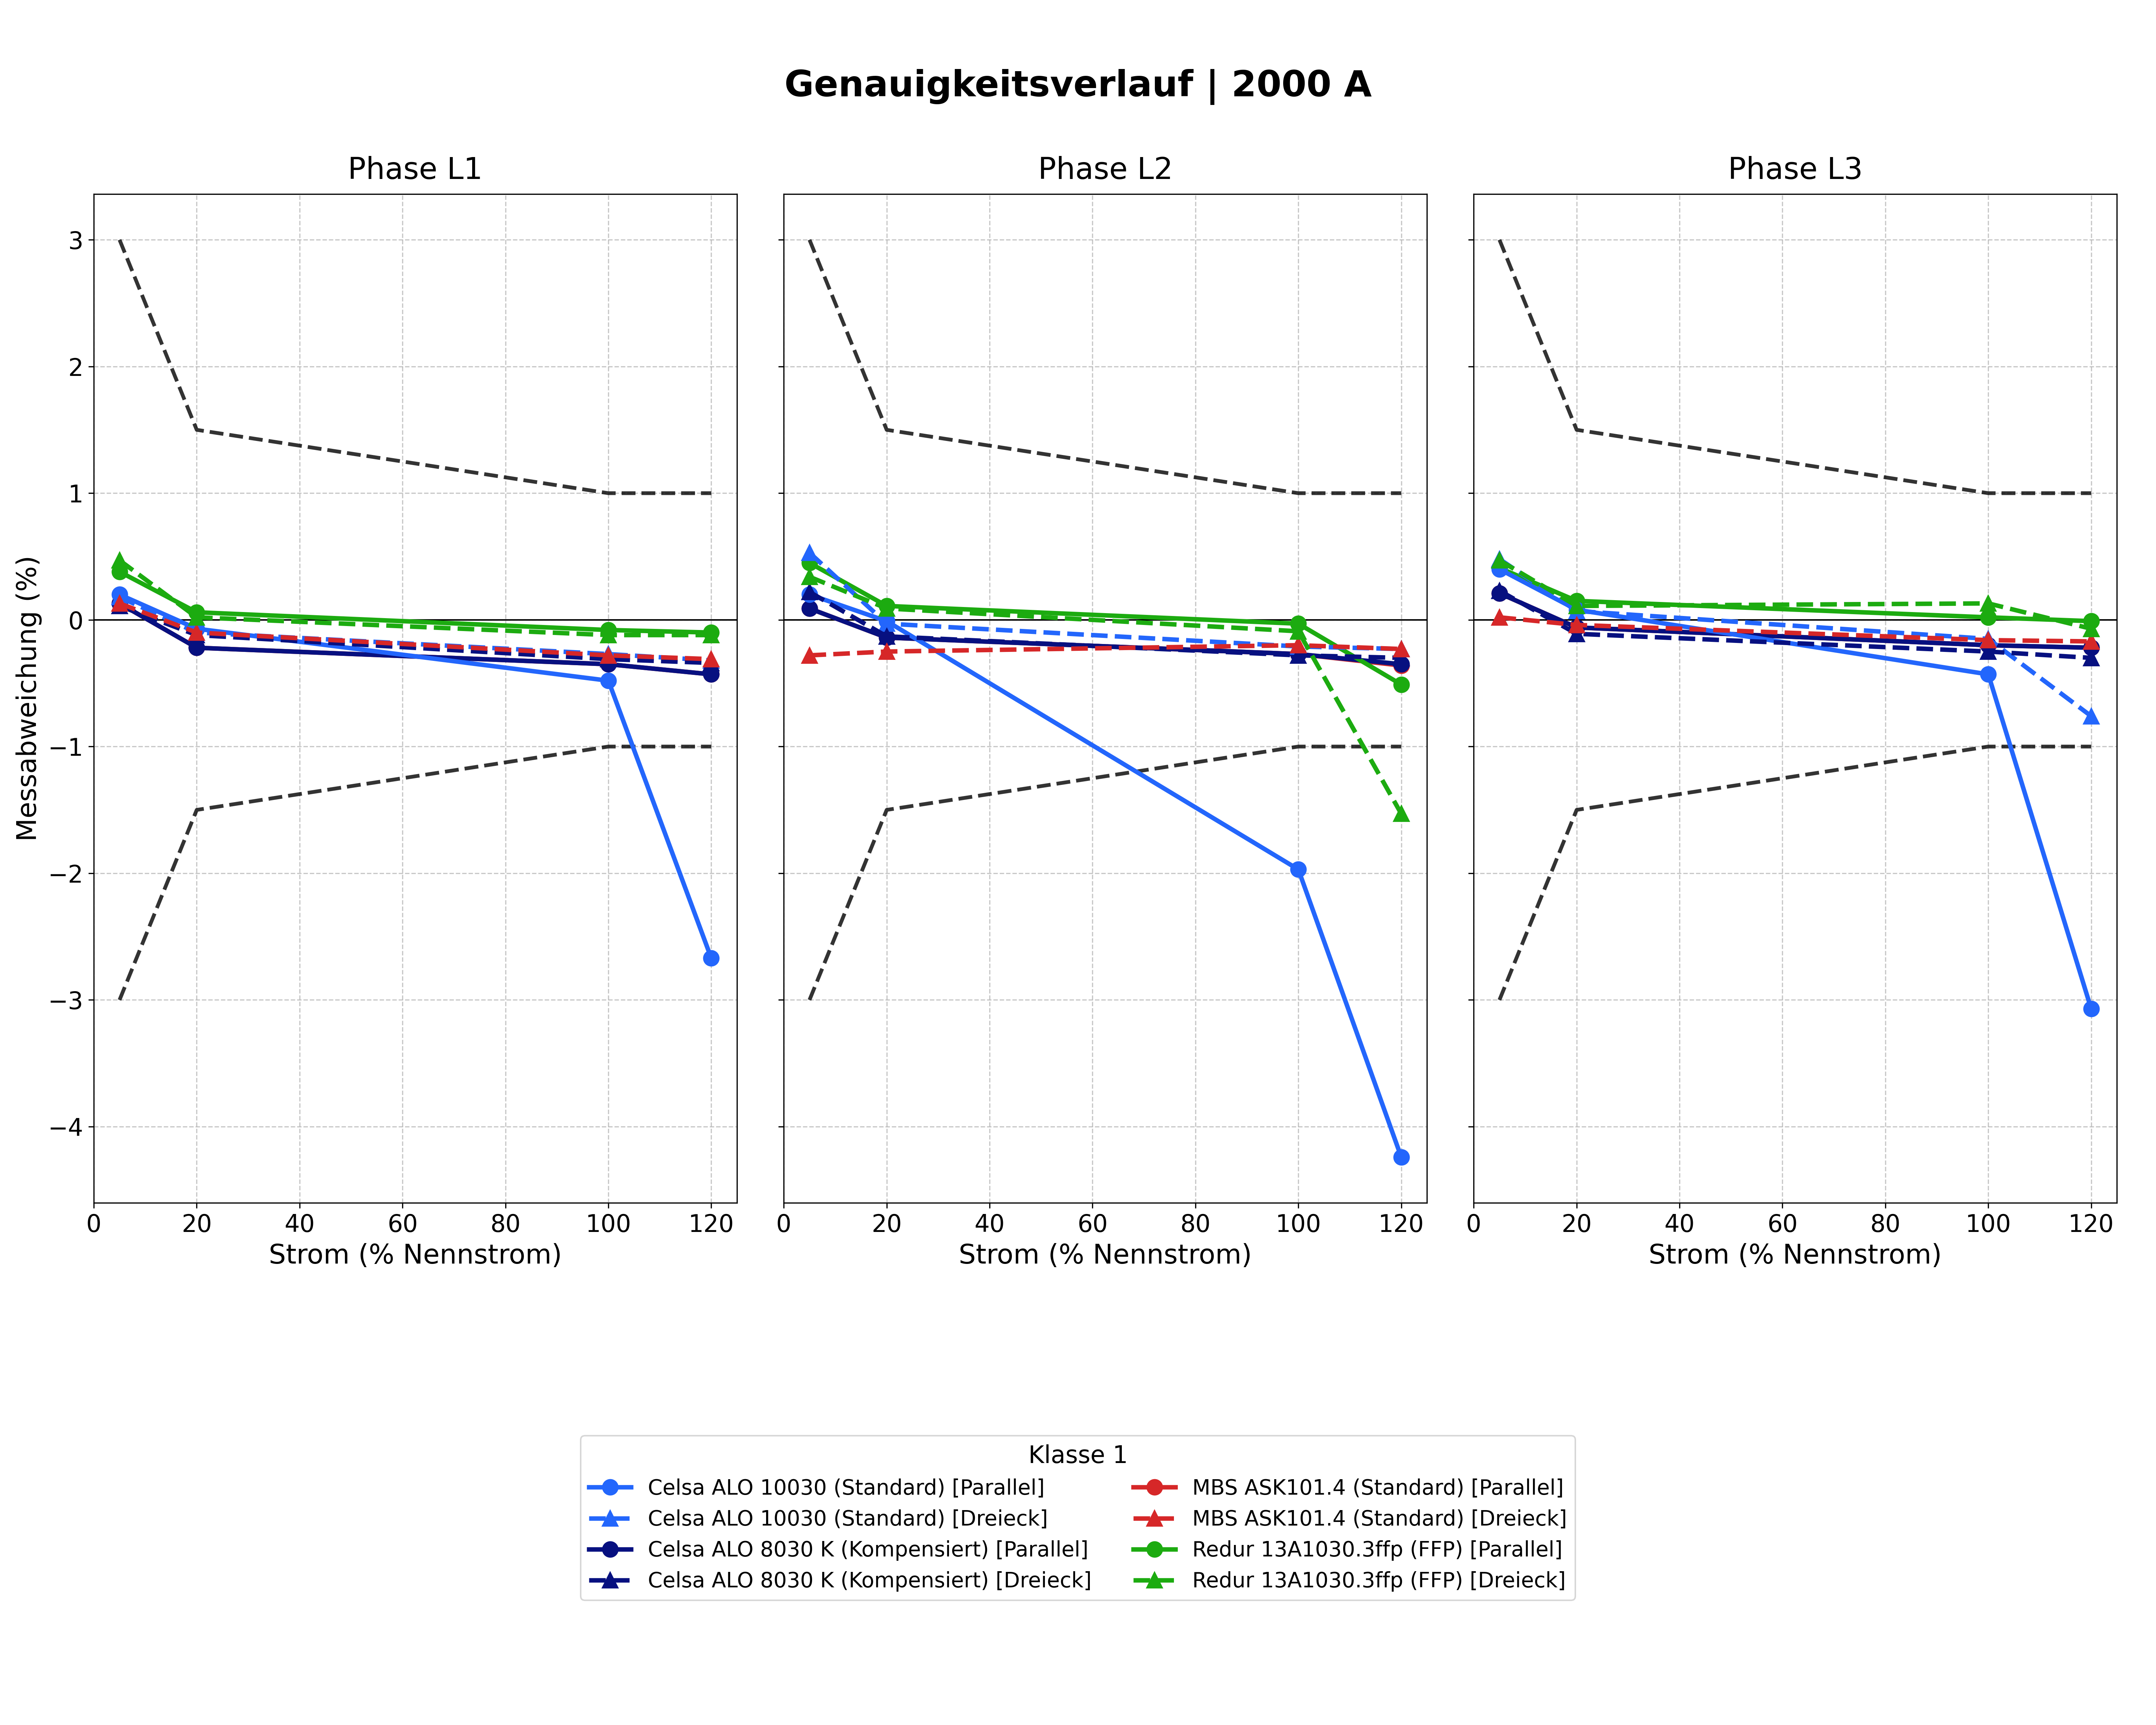
\includegraphics[width=1.0\textwidth]{03_Ressourcen/dia_neu/verlauf/mes_2000A_verlauf.png}
    \caption{Übersetzungsmessabweichung \gls{sym:epsilon} bei \SI{2000}{A}: Vergleich von Parallel- und Dreiecksanordnung (Phasen L1--L3)}
    \label{dia:2000A_zusammenfassung}
\end{diagram}

Eine bauliche Besonderheit weist der \textit{Redur~13A1030.ffp} auf. Wie in Abbildung~\ref{fig:wandler_fremdfeldprotektor} zu erkennen ist, sind die Fremdfeldprotektoren (\gls{ffp}) seitlich an den Flanken des Gehäuses angeordnet. Damit wird der Eisenkern gegenüber magnetischen Streufeldern benachbarter Leiter insbesondere dann wirksam abgeschirmt, wenn diese seitlich positioniert sind. In der parallelen Leiterführung ergeben sich folgerichtig normkonforme Messergebnisse, da die Beeinflussung durch die Nachbarphasen deutlich reduziert wird.

\begin{figure}[H]
    \centering
    \includegraphics[width=1.0\textwidth]{03_Ressourcen/Bilder/wandler_redur_2000A_dreiecksmessung_beschriftet.pdf}
    \caption{Seitliche Fremdfeldprotektoren am \textit{Redur~Wandler}}
    \label{fig:wandler_fremdfeldprotektor}
\end{figure}

Die Grenzen dieser Schirmung zeigen sich in der Dreieckskonfiguration. Die vollständigen Messergebnisse sind in Tabelle~\ref{tab:messergebnisse_redur_2000A} im Anhang aufgeführt. Bei \SI{120}{\percent} des Nennstroms weist Phase L2 eine Übersetzungsmessabweichung \gls{sym:epsilon} von \num{-1,50}\,\% auf und liegt damit außerhalb der zulässigen Toleranz der Genauigkeitsklasse \num{1}. Ursächlich ist die fehlende magnetische Schirmung auf der Rückseite des Wandlergehäuses. In der Dreiecksgeometrie können Magnetfelder benachbarter Leiter an dieser ungeschützten Stelle in den Eisenkern einkoppeln und ihn partiell sättigen. Im selben Lastpunkt bleibt Phase L1 mit einer Abweichung von lediglich \num{-0,10}\,\% hingegen deutlich innerhalb der Normgrenzen.

Ein konträres Verhalten zeigt der \textit{Celsa~ALO~10030}. Die Messergebnisse in Tabelle~\ref{tab:messergebnisse_celsa_2000A} im Anhang belegen in der Parallelanordnung deutliche Genauigkeitseinbußen. Bereits bei Nennstrom \gls{sym:In} verletzt Phase L2 mit \num{-2,00}\,\% den zulässigen Grenzwert. Bei \SI{120}{\percent} Überlast steigt \gls{sym:epsilon} weiter auf \num{-4,20}\,\% an. Auch die Außenleiter L1 und L3 zeigen in der Parallelanordnung bei \SI{120}{\percent} Last mit \num{-2,70}\,\% beziehungsweise \num{-3,10}\,\% erkennbare Fehler. Wird die Leitergeometrie zur Dreiecksanordnung geändert, verbessert sich das Verhalten deutlich. Der Fehler der Phase L2 reduziert sich bei \SI{120}{\percent} Last auf \num{-0,20}\,\%. Entsprechend sind in Abbildung~\ref{dia:2000A_zusammenfassung} für die Parallelanordnung des \textit{Celsa~ALO~10030} deutlich stärkere Abfälle der Messkurven zu erkennen, insbesondere ab etwa \SI{20}{\percent} des Nennstroms. Die Dreiecksanordnung verläuft dagegen weitgehend linear und bleibt im Toleranzband.

Zur kompakten Gegenüberstellung der Geometrieeffekte über den gesamten Lastbereich zeigt Abbildung~\ref{dia:2000A_bereichsanalyse} eine \textit{Bereichsanalyse} des mittleren absoluten Fehlers. Dazu werden die Absolutwerte der Übersetzungsmessabweichung \gls{sym:epsilon} über alle drei Phasen gemittelt und getrennt nach Niederstrom (\SI{5}{\percent}--\SI{50}{\percent}), Nennstrom (\SI{80}{\percent}--\SI{100}{\percent}) sowie Überlast (\SI{120}{\percent}) ausgewertet. Beim \textit{Celsa~ALO~10030} zeigt die Parallelanordnung einen ausgeprägten Anstieg im Hochlastbereich (\num{3,33}\,\% bei Überlast), während die Dreiecksanordnung den Überlastfehler auf \num{0,44}\,\% reduziert. Der \textit{Redur~13A1030.3ffp} weist im Nieder- und Nennstrombereich in beiden Geometrien ähnliche Fehlerwerte (\(\approx\num{0,25}\,\%\) bzw. \(\approx\num{0,03}\,\%\)) auf; bei \SI{120}{\percent} bleibt die Parallelanordnung mit \num{0,21}\,\% günstiger als die Dreiecksanordnung mit \num{0,57}\,\%. Die beiden übrigen Modelle (\textit{Celsa~ALO~8030~K}, \textit{MBS~ASK~101.4}) verbleiben über alle Lastbereiche unter \num{0,35}\,\% und sind damit nur schwach von der Leitergeometrie abhängig.

\begin{diagram}[H]
    \centering
    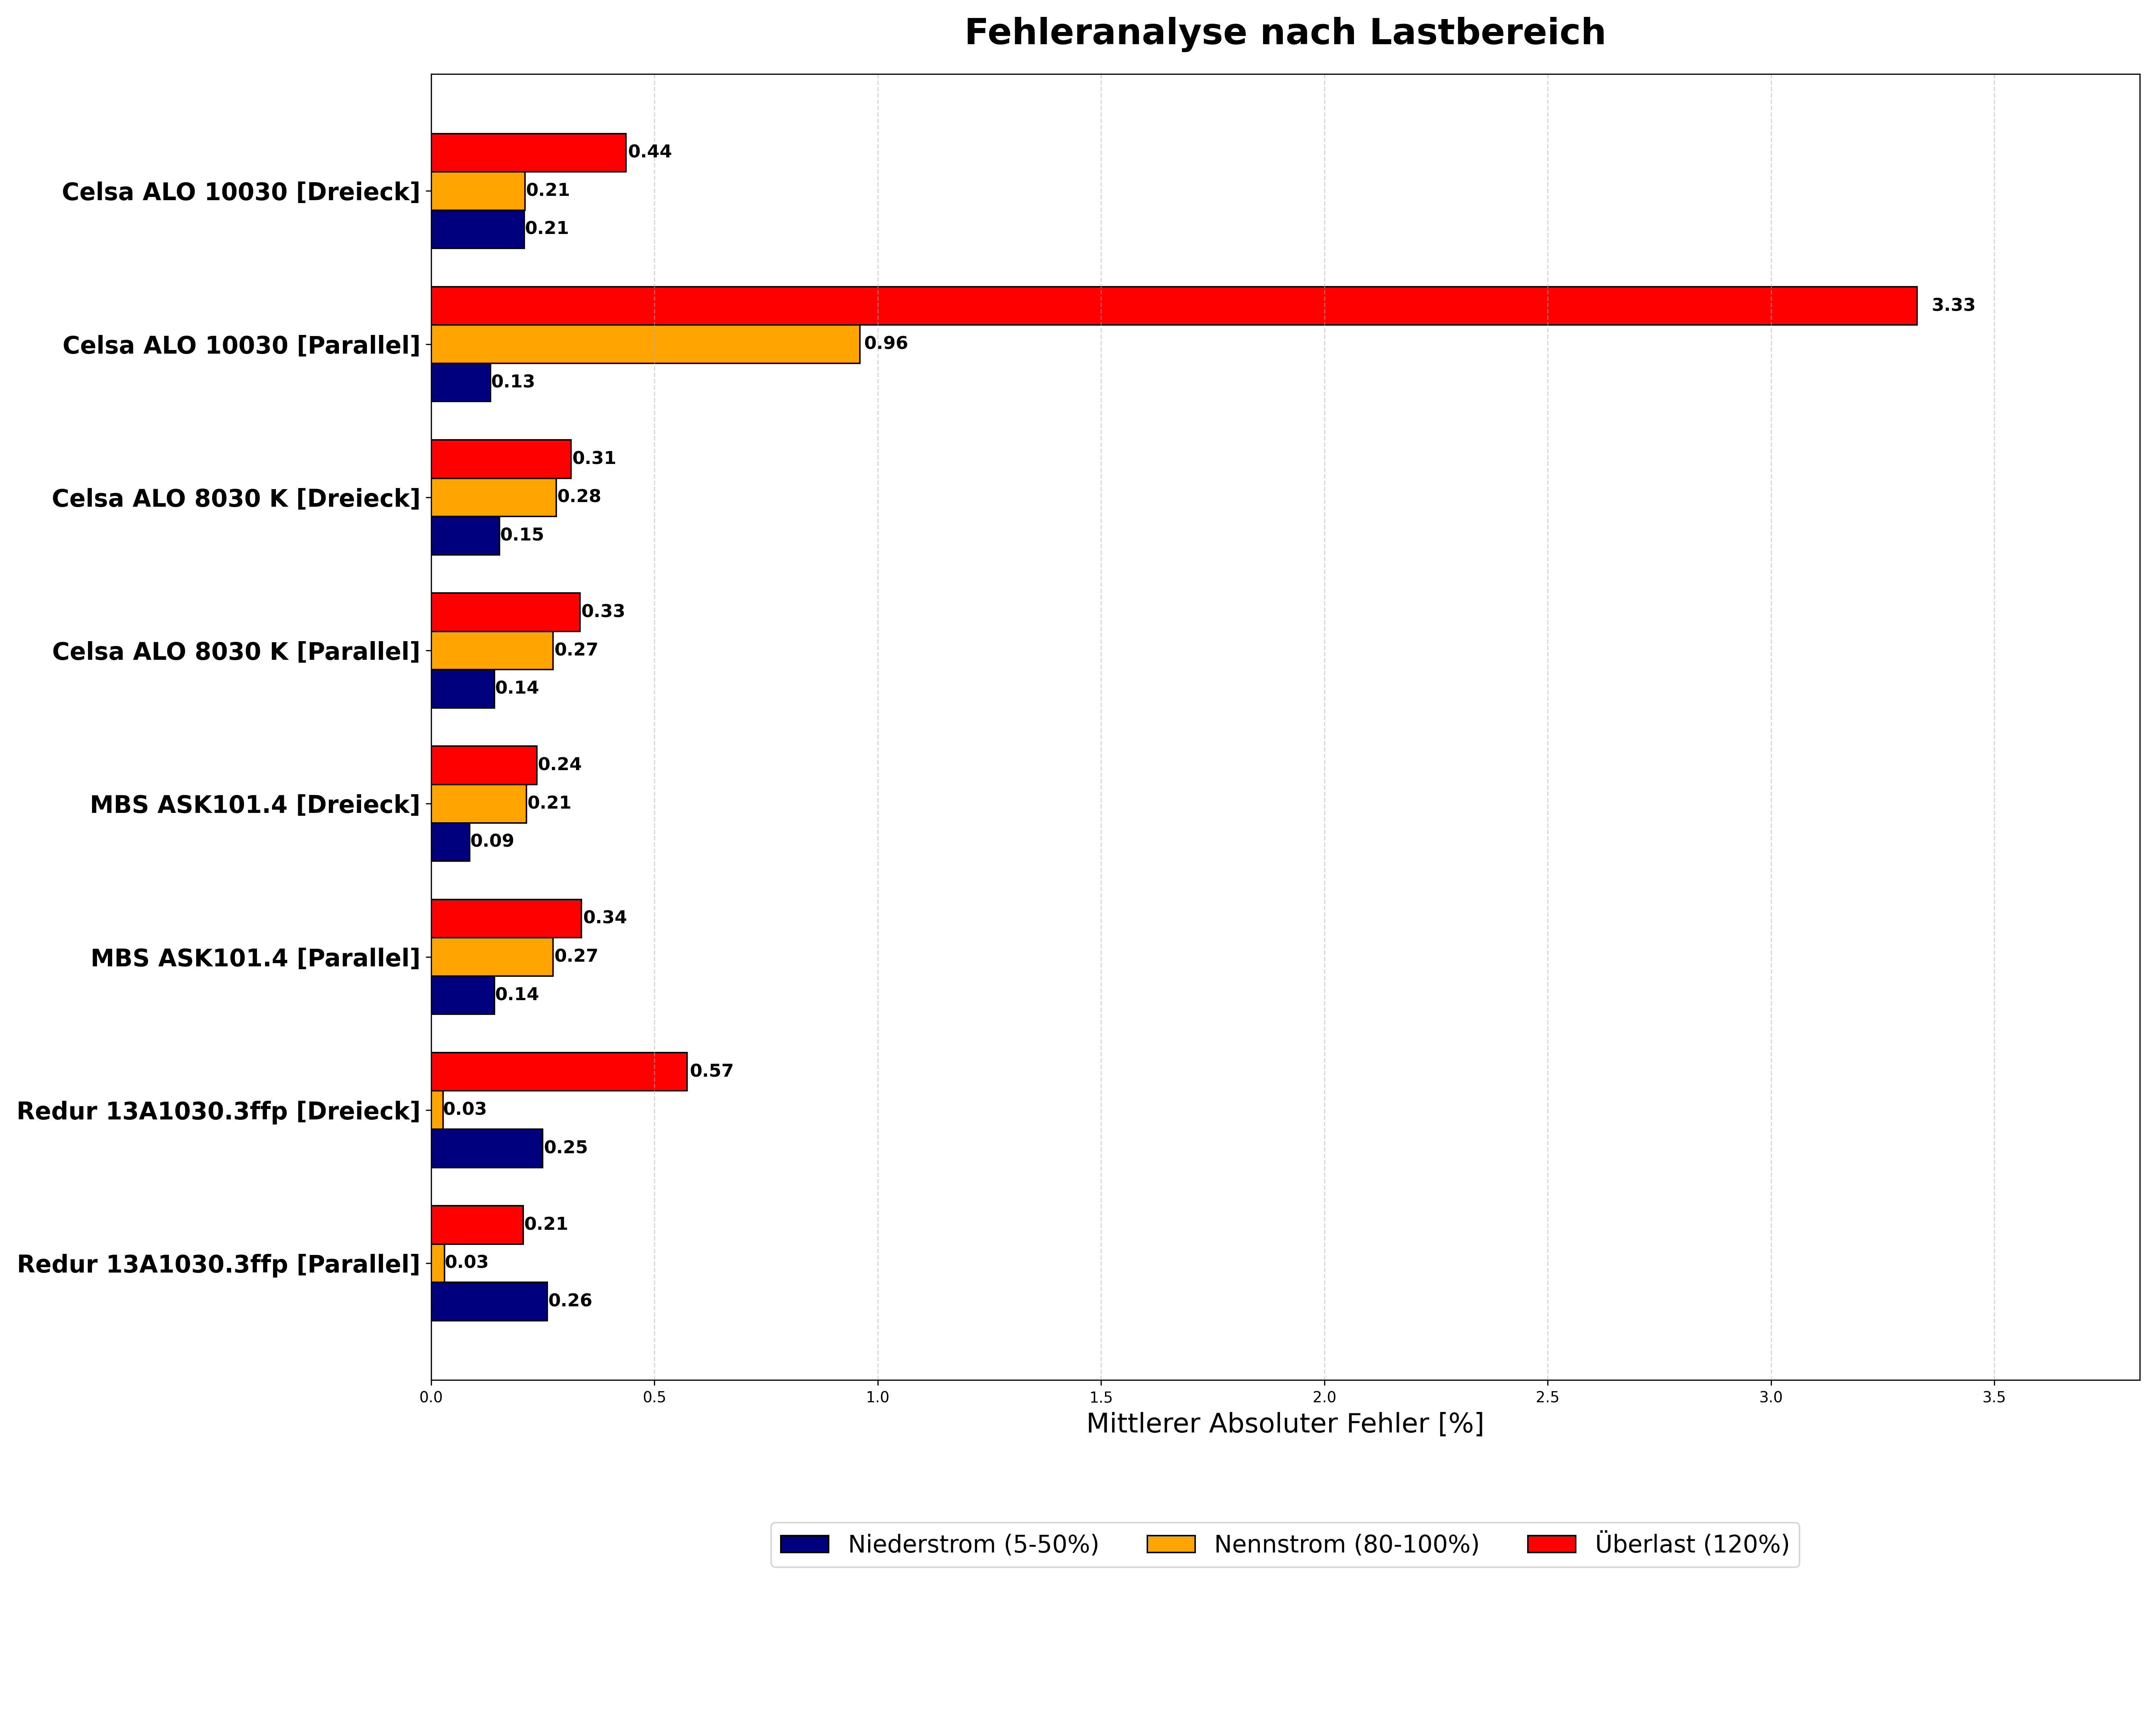
\includegraphics[width=1.0\textwidth]{03_Ressourcen/dia_neu/bereichs_analyse/mes_2000A_bereichs_analyse.png}
    \caption{Fehleranalyse nach Lastbereich bei \SI{2000}{A}: mittlerer absoluter Fehler im Niederstrom-, Nennstrom- und Überlastbereich (Vergleich Parallel- und Dreiecksanordnung)}
    \label{dia:2000A_bereichsanalyse}
\end{diagram}

Im Gegensatz zu den beschriebenen Abweichungen zeigen der \textit{Celsa~ALO~8030~K} und der \textit{MBS~ASK~101.4} eine hohe Stabilität gegenüber externen Feldern. Beim \textit{Celsa~ALO~8030~K} ist dies auf die Bauweise als kompensierter Wandler zurückzuführen, wie in Abschnitt~\ref{sec:kompensationswicklungen} erläutert wird. Tabelle~\ref{tab:messergebnisse_celsa8030_2000A} im Anhang fasst die Ergebnisse zusammen. Selbst unter Volllast und Überstrom bleiben alle Phasen in beiden geometrischen Anordnungen innerhalb der Klasse \num{1}. Die maximale Abweichung tritt in der Parallelanordnung bei Phase L1 mit \num{-0,40}\,\% auf.

Ein ähnlich robustes Verhalten zeigt der \textit{MBS~ASK~101.4}. Tabelle~\ref{tab:messergebnisse_mbs_2000A} im Anhang weist keine signifikanten Einflüsse der Leiteranordnung aus. Die Messwerte liegen insgesamt auf einem Niveau, das mit dem \textit{Celsa~ALO~8030~K} vergleichbar ist. In der Dreiecksanordnung erreicht Phase L1 bei \SI{120}{\percent} Last beispielsweise eine Abweichung von \num{-0,30}\,\% und bestätigt damit die geringe Empfindlichkeit dieses Modells gegenüber den untersuchten Leitergeometrien.



\subsubsection{Einfluss der Leitergeometrie auf das Sättigungsverhalten bei \SI{2500}{A}}
\label{sec:analyse_messreihe_2500A}

Die Analyse der Messreihe bei einem Nennstrom \gls{sym:In} von \SI{2500}{A} zeigt einen ausgeprägten Einfluss der Leitergeometrie auf unterschiedliche Wandlertechnologien. Im Mittelpunkt steht der Vergleich zwischen dem kompensierten Wandler \textit{Celsa~ALO~10050~K} und dem Standardwandler \textit{Celsa~ALO~10030} im Hinblick auf ihre Stabilität in Parallel- und Dreiecksanordnung. Abbildung~\ref{dia:2500A_zusammenfassung} stellt die Messabweichungen für die Phasen L1 bis L3 über dem Lastbereich dar und macht die unterschiedlichen Verläufe beider Wandlerkonzepte sichtbar. Die zugehörigen Messwerte sind im Anhang in den Tabellen~\ref{tab:messergebnisse_celsa10050_2500A_alle} und \ref{tab:messergebnisse_celsa10030_2500A_alle} dokumentiert.



\begin{diagram}[H]
    \centering
    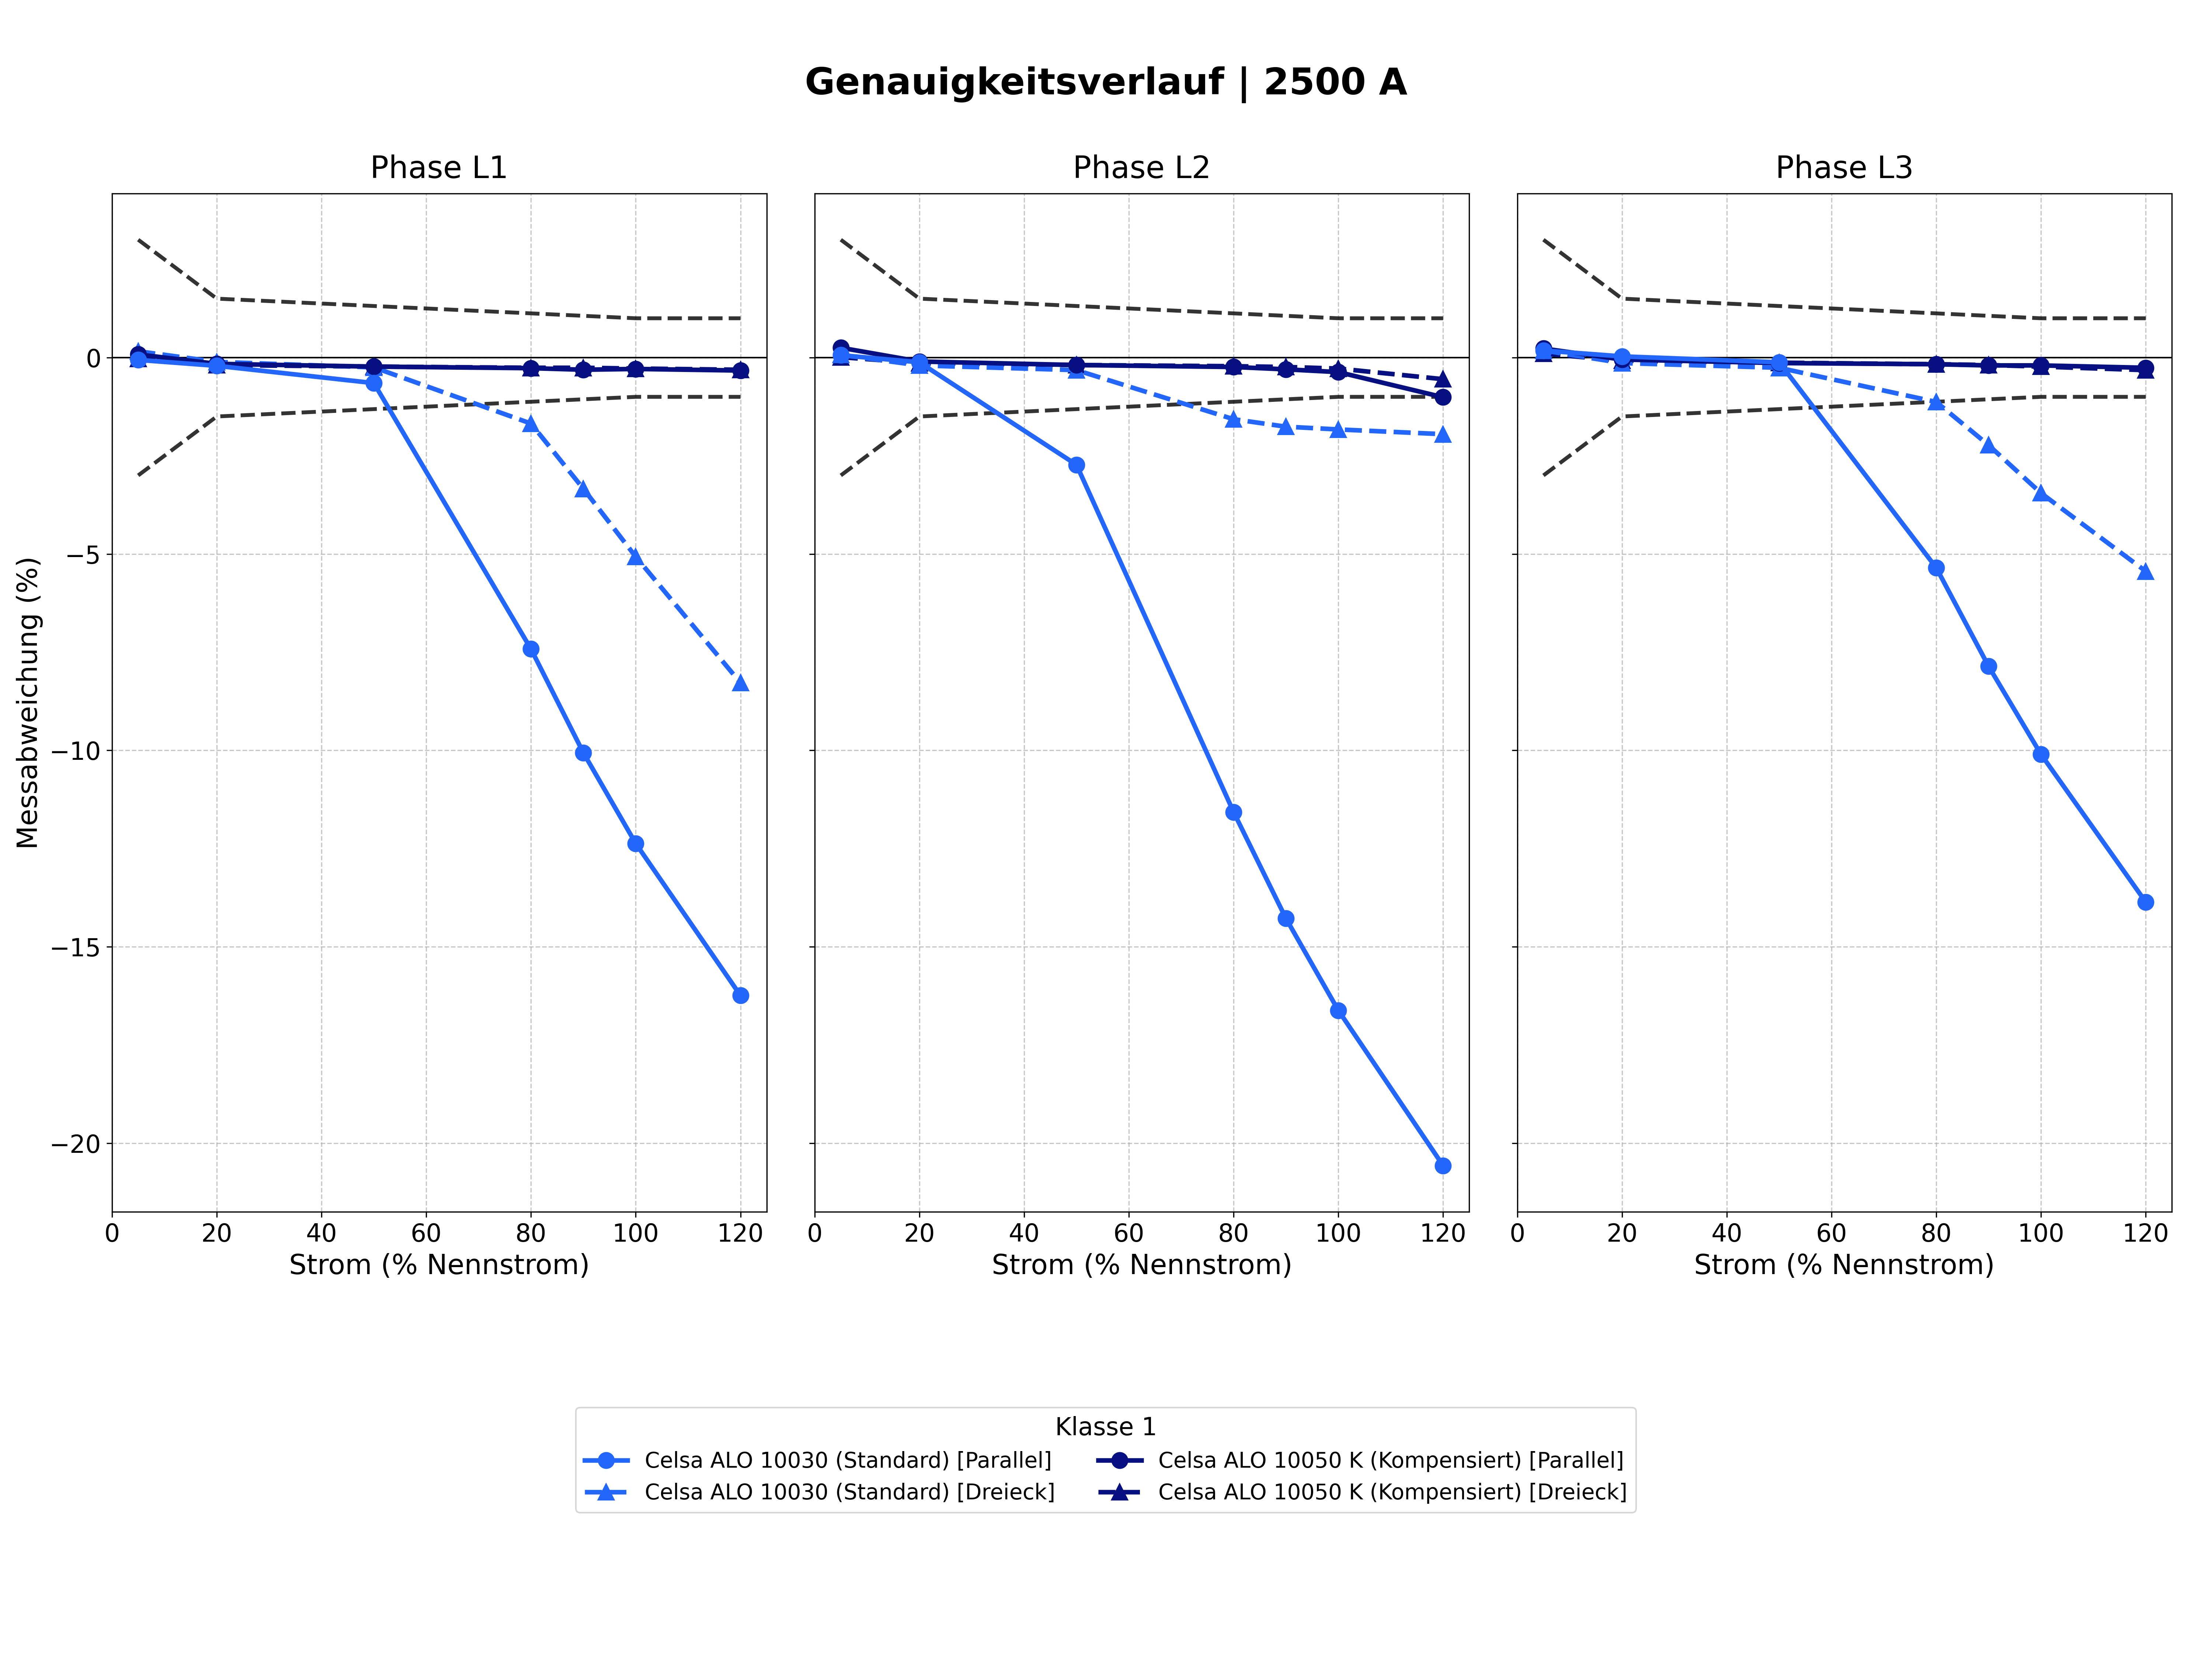
\includegraphics[width=1.0\textwidth]{03_Ressourcen/dia_neu/verlauf/mes_2500A_verlauf.png}
    \caption{Übersetzungsmessabweichung \gls{sym:epsilon} bei \SI{2500}{A}: Vergleich von Parallel- und Dreiecksanordnung (Phasen L1--L3)}
    \label{dia:2500A_zusammenfassung}
\end{diagram}

Die Messergebnisse des kompensierten Wandlers \textit{Celsa~ALO~10050~K} zeigen über weite Bereiche eine hohe Genauigkeit. In der Parallelanordnung liegt der Wandler nahezu durchgehend innerhalb der normativen Vorgaben, wie Tabelle~\ref{tab:messergebnisse_celsa10050_2500A_alle} im Anhang ausweist. Eine Ausnahme bildet die Phase L2 im Überlastbereich bei \SI{120}{\percent} des Nennstroms \gls{sym:In}. Dort ergibt sich eine Übersetzungsmessabweichung \gls{sym:epsilon} von rund \num{-1,00}\,\%, was einem absoluten Fehlstrom von circa \num{30,00}\,\unit{A} entspricht.

In der Dreiecksanordnung reduziert sich dieser Messfehler auf etwa \num{-0,55}\,\%, wodurch die Genauigkeitsklasse \num{1} wieder eingehalten wird. Damit zeigt sich, dass auch ein kompensierter Wandler nicht vollständig unempfindlich gegenüber externen Magnetfeldern ist, die Auswirkungen jedoch im Vergleich zur Standardtechnologie gering bleiben.

Abbildung~\ref{dia:2500A_bereichsanalyse} ergänzt die Kurven aus Abbildung~\ref{dia:2500A_zusammenfassung} durch eine \textit{Bereichsanalyse} des mittleren absoluten Fehlers. Der Standardwandler \textit{Celsa~ALO~10030} zeigt dabei, dass die Abweichungen nahezu ausschließlich im oberen Lastbereich auftreten: Während der Niederstromfehler in beiden Geometrien unter \num{0,5}\,\% bleibt, steigt der mittlere Fehler im Nennstrombereich in Parallelanordnung auf \num{10,63}\,\% und im Überlastpunkt auf \num{16,89}\,\%. Die Dreiecksanordnung reduziert diese Werte auf \num{2,45}\,\% beziehungsweise \num{5,22}\,\%, verhindert die Sättigung jedoch nicht vollständig. Der kompensierte \textit{Celsa~ALO~10050~K} verbleibt demgegenüber über alle Lastbereiche in beiden Geometrien unter \num{0,55}\,\% und bestätigt damit die Wirksamkeit der Kompensation im Hochlastbereich.

\begin{diagram}[H]
    \centering
    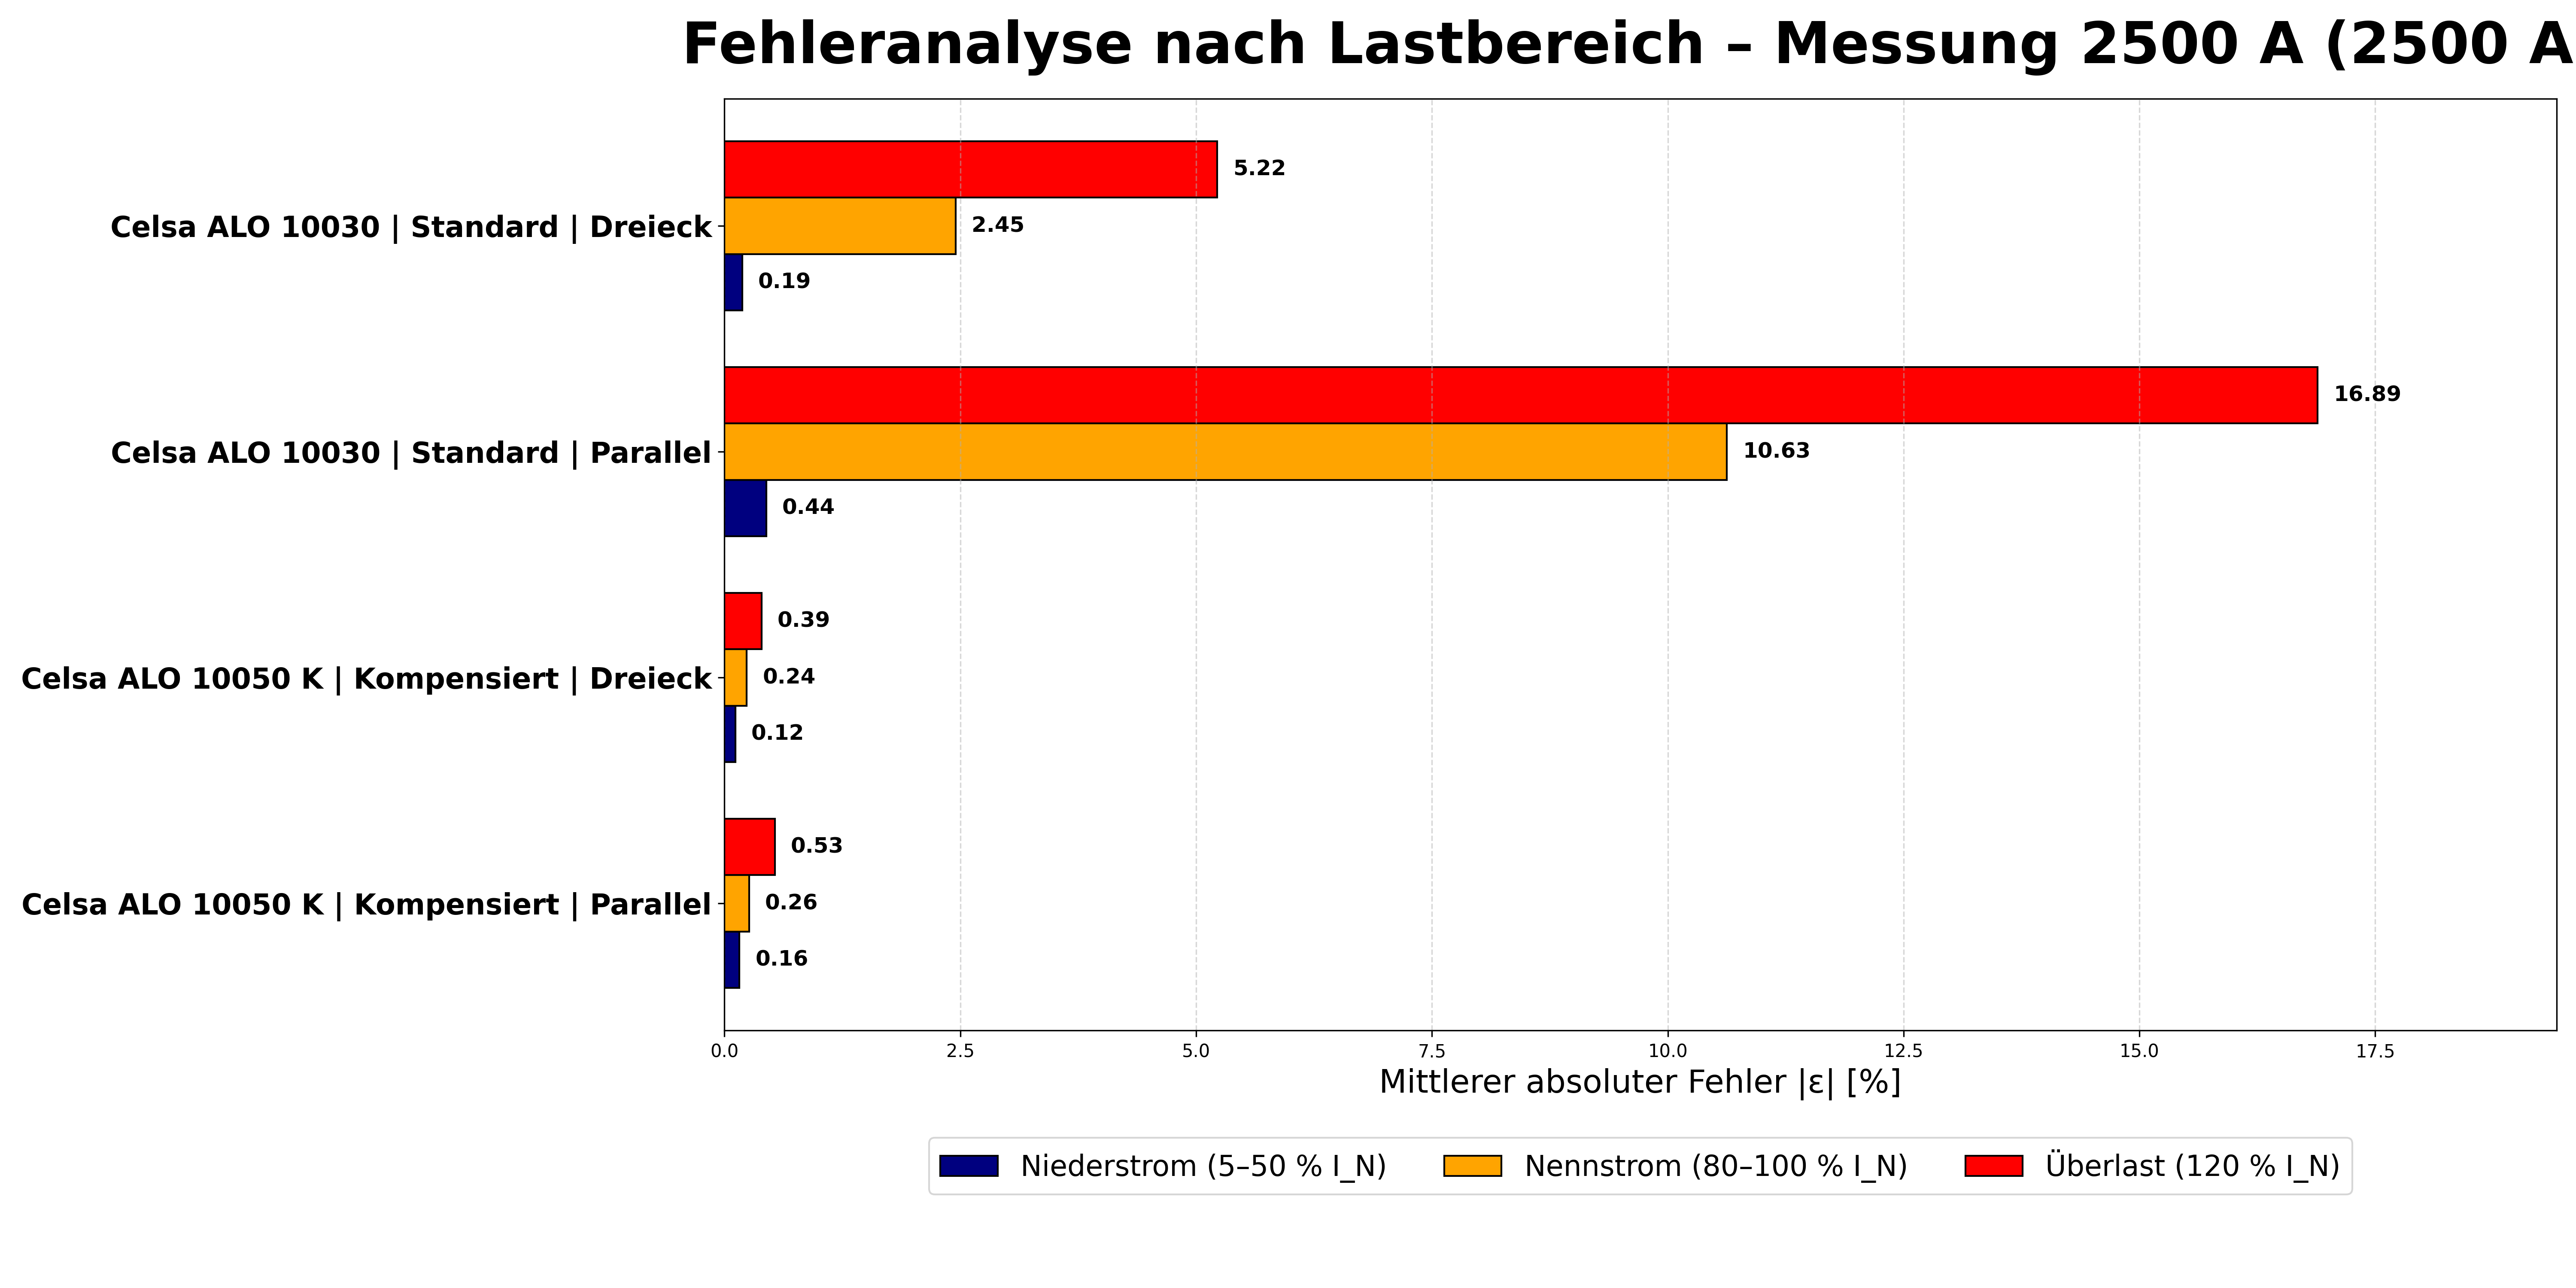
\includegraphics[width=1.0\textwidth]{03_Ressourcen/dia_neu/bereichs_analyse/mes_2500A_bereichs_analyse.png}
    \caption{Fehleranalyse nach Lastbereich bei \SI{2500}{A}: mittlerer absoluter Fehler im Niederstrom-, Nennstrom- und Überlastbereich (Vergleich Parallel- und Dreiecksanordnung)}
    \label{dia:2500A_bereichsanalyse}
\end{diagram}

Der nicht kompensierte Standardwandler \textit{Celsa~ALO~10030} zeigt im Hochlastbereich erhebliche Abweichungen, die auf eine beginnende magnetische Sättigung hindeuten. Die vollständigen Messwerte sind in Tabelle~\ref{tab:messergebnisse_celsa10030_2500A_alle} im Anhang aufgeführt. In der Parallelanordnung steigt der Fehler bereits ab \SI{50}{\percent} des Nennstroms \gls{sym:In} deutlich an. Bei \SI{100}{\percent} Last liegen die Abweichungen \gls{sym:epsilon} zwischen \num{-10,00}\,\% und \num{-16,00}\,\%. Bei \SI{120}{\percent} Last werden in einzelnen Phasen Fehlströme in der Größenordnung mehrerer hundert Ampere erreicht, was den deutlichen Einbruch der Messgenauigkeit im Überlastbereich bestätigt.

Trotz der betrachteten Leitergeometrien wird die Genauigkeitsklasse \num{1} im Hochlastbereich nicht eingehalten. Die verbleibende Abweichung deutet auf eine grundsätzliche Unterdimensionierung des magnetischen Kreises hin. Ein Vergleich mit den Ergebnissen aus Abschnitt~\ref{sec:analyse_messreihe_2000A} stützt diese Einordnung, da dieser Wandlertyp bereits dort Sättigungstendenzen im Bereich des Nennstroms zeigte. Für das hier untersuchte \SI{2500}{A}-Modell ist zudem erkennbar, dass der starke Fehleranstieg bereits bei \SI{80}{\percent} der Nennlast einsetzt, was einem Primärstrom \gls{sym:I_p} von \SI{2000}{A} entspricht.

Damit fällt der Sättigungsbeginn mit den Beobachtungen der vorherigen Messreihe zusammen. Dies legt nahe, dass der magnetische Kreis dieses Bauteils für Ströme oberhalb von \SI{2000}{A} nicht ausreichend dimensioniert ist. Dieser empirische Befund steht im Einklang mit den Zusammenhängen aus Gleichung~\ref{eq:b_phi_relation}. Wie dort hergeleitet, führt ein zu geringer Eisenquerschnitt \gls{sym:A_Fe} dazu, dass sich der magnetische Fluss auf eine zu kleine Fläche konzentriert. Dadurch steigt die resultierende Flussdichte \gls{sym:B_res} an und die Sättigungsgrenze des Materials wird frühzeitig erreicht.

\begin{table}[H]
    \centering
    \caption{Abschätzung des effektiven Eisenquerschnitts $A_{Fe}$}
    \label{tab:wandler_querschnitt}
    \begin{tabular}{
            l
            c
            c
            S[table-format=2.2]
        }
        \toprule
        {Modell}                   & {Maße ($H \times T$)} & {Füllfaktor} & {Querschnitt $A_{Fe}$ [\unit{cm^2}]} \\
        \midrule
        \textit{Celsa~ALO~10030}   & $31 \times \SI{144}{mm}$   & 0.7          & 31.25                        \\
        \textit{Celsa~ALO~10050~K} & $50 \times \SI{145}{mm}$   & 0.7          & 50.75                        \\
        \bottomrule
    \end{tabular}
\end{table}

Tabelle~\ref{tab:wandler_querschnitt} untermauert diese Einordnung durch eine Abschätzung des magnetisch wirksamen Eisenquerschnitts \gls{sym:A_Fe}. Da die exakten Innenmaße der vergossenen Wandler nicht bekannt sind, stellt die Berechnung eine Näherung an die tatsächlichen physikalischen Gegebenheiten dar. Basierend auf den äußeren Gehäuseabmessungen (Höhe $H$ und Tiefe $T$) wird ein Faktor von \num{0,7} angesetzt. Dieser Schätzwert versucht, den realen Eisenquerschnitt unter Berücksichtigung der nicht magnetischen Bestandteile wie Gehäusewandungen, Isolation und Sekundärwicklung bestmöglich abzubilden.

Die Abschätzung zeigt, dass dem Typ \textit{Celsa~ALO~10050~K} mit rund \num{50,75}\,\unit{cm^2} eine signifikant größere Querschnittsfläche zur Verfügung steht als dem Standardwandler \textit{Celsa~ALO~10030} mit lediglich \num{31,25}\,\unit{cm^2}. Der um circa \num{60}\,\% größere Eisenquerschnitt ermöglicht eine deutlich geringere Flussdichte bei gleicher induzierter Spannung, was die spätere Sättigung des kompensierten Wandlers physikalisch erklärt.


\subsubsection{Einfluss von Geometrie und Bürde bei \SI{3000}{A}}
\label{sec:analyse_messreihe_3000A}

Die Messreihe bei \SI{3000}{A} dient als Fallstudie zur Charakterisierung des Wandlerverhaltens im Grenzbereich. Untersucht wird der Standardwandler \textit{Celsa~ALO~12070} im Vergleich zur kompensierten Ausführung \textit{Celsa~ALO~12070~K} unter dem Einfluss der Leitergeometrie. Zusätzlich wird geprüft, ob eine Reduktion des sekundären Bürdenwiderstands \gls{sym:RB} die Sättigungseffekte in der kritischen Parallelanordnung abschwächen kann. Die zugehörigen Messwerte sind im Anhang in den Tabellen~\ref{tab:messergebnisse_celsa12070_3000A_alle}, \ref{tab:messergebnisse_celsa12070_3000A_asym} und \ref{tab:messergebnisse_celsa12070_3000A_min} aufgeführt.

\paragraph{Vergleich der Wandlertechnologien und Geometrien}

Abbildung~\ref{dia:3000A_zusammenfassung} zeigt die Fehlerverläufe beider Wandlertypen in Dreiecks- und Parallelanordnung. Die gestrichelten Begrenzungslinien markieren den zulässigen Toleranzbereich der Genauigkeitsklasse \num{1}. Beim Standardwandler \textit{Celsa~ALO~12070} fällt insbesondere Phase L2 auf. Wie Tabelle~\ref{tab:messergebnisse_celsa12070_3000A_alle} im Anhang zeigt, unterschreitet der Messwert bei \SI{80}{\percent} des Nennstroms \gls{sym:In} mit \num{-1,10}\,\% den Grenzwert. Mit weiter steigender Last nimmt der Fehler zu und erreicht bei \SI{120}{\percent} einen Wert von \num{-5,40}\,\%. Dies entspricht einem absoluten Fehlstrom von rund \num{195,30}\,\unit{A}.

Der kompensierte Typ \textit{Celsa~ALO~12070~K} zeigt demgegenüber eine deutlich stabilere Erfassung von Phase L2, sodass die Normeinhaltung im betrachteten Bereich gewährleistet ist. Im Überlastbereich tritt in der Parallelanordnung eine positive Abweichung \gls{sym:epsilon} auf. Dies deutet auf Effekte hin, die sich wie eine Unterbürdung infolge veränderter Flussverhältnisse im Kern auswirken können. Die Außenleiter L1 und L3 verhalten sich in beiden Konfigurationen weitgehend ähnlich und verbleiben im Toleranzbereich. Der Vergleich der Geometrien beim kompensierten Wandler zeigt den Unterschied vor allem bei Phase L2. Der Fehler liegt in der Parallelanordnung bei \num{0,90}\,\% und in der Dreiecksanordnung bei \num{0,10}\,\%.

\begin{diagram}[H]
    \centering
    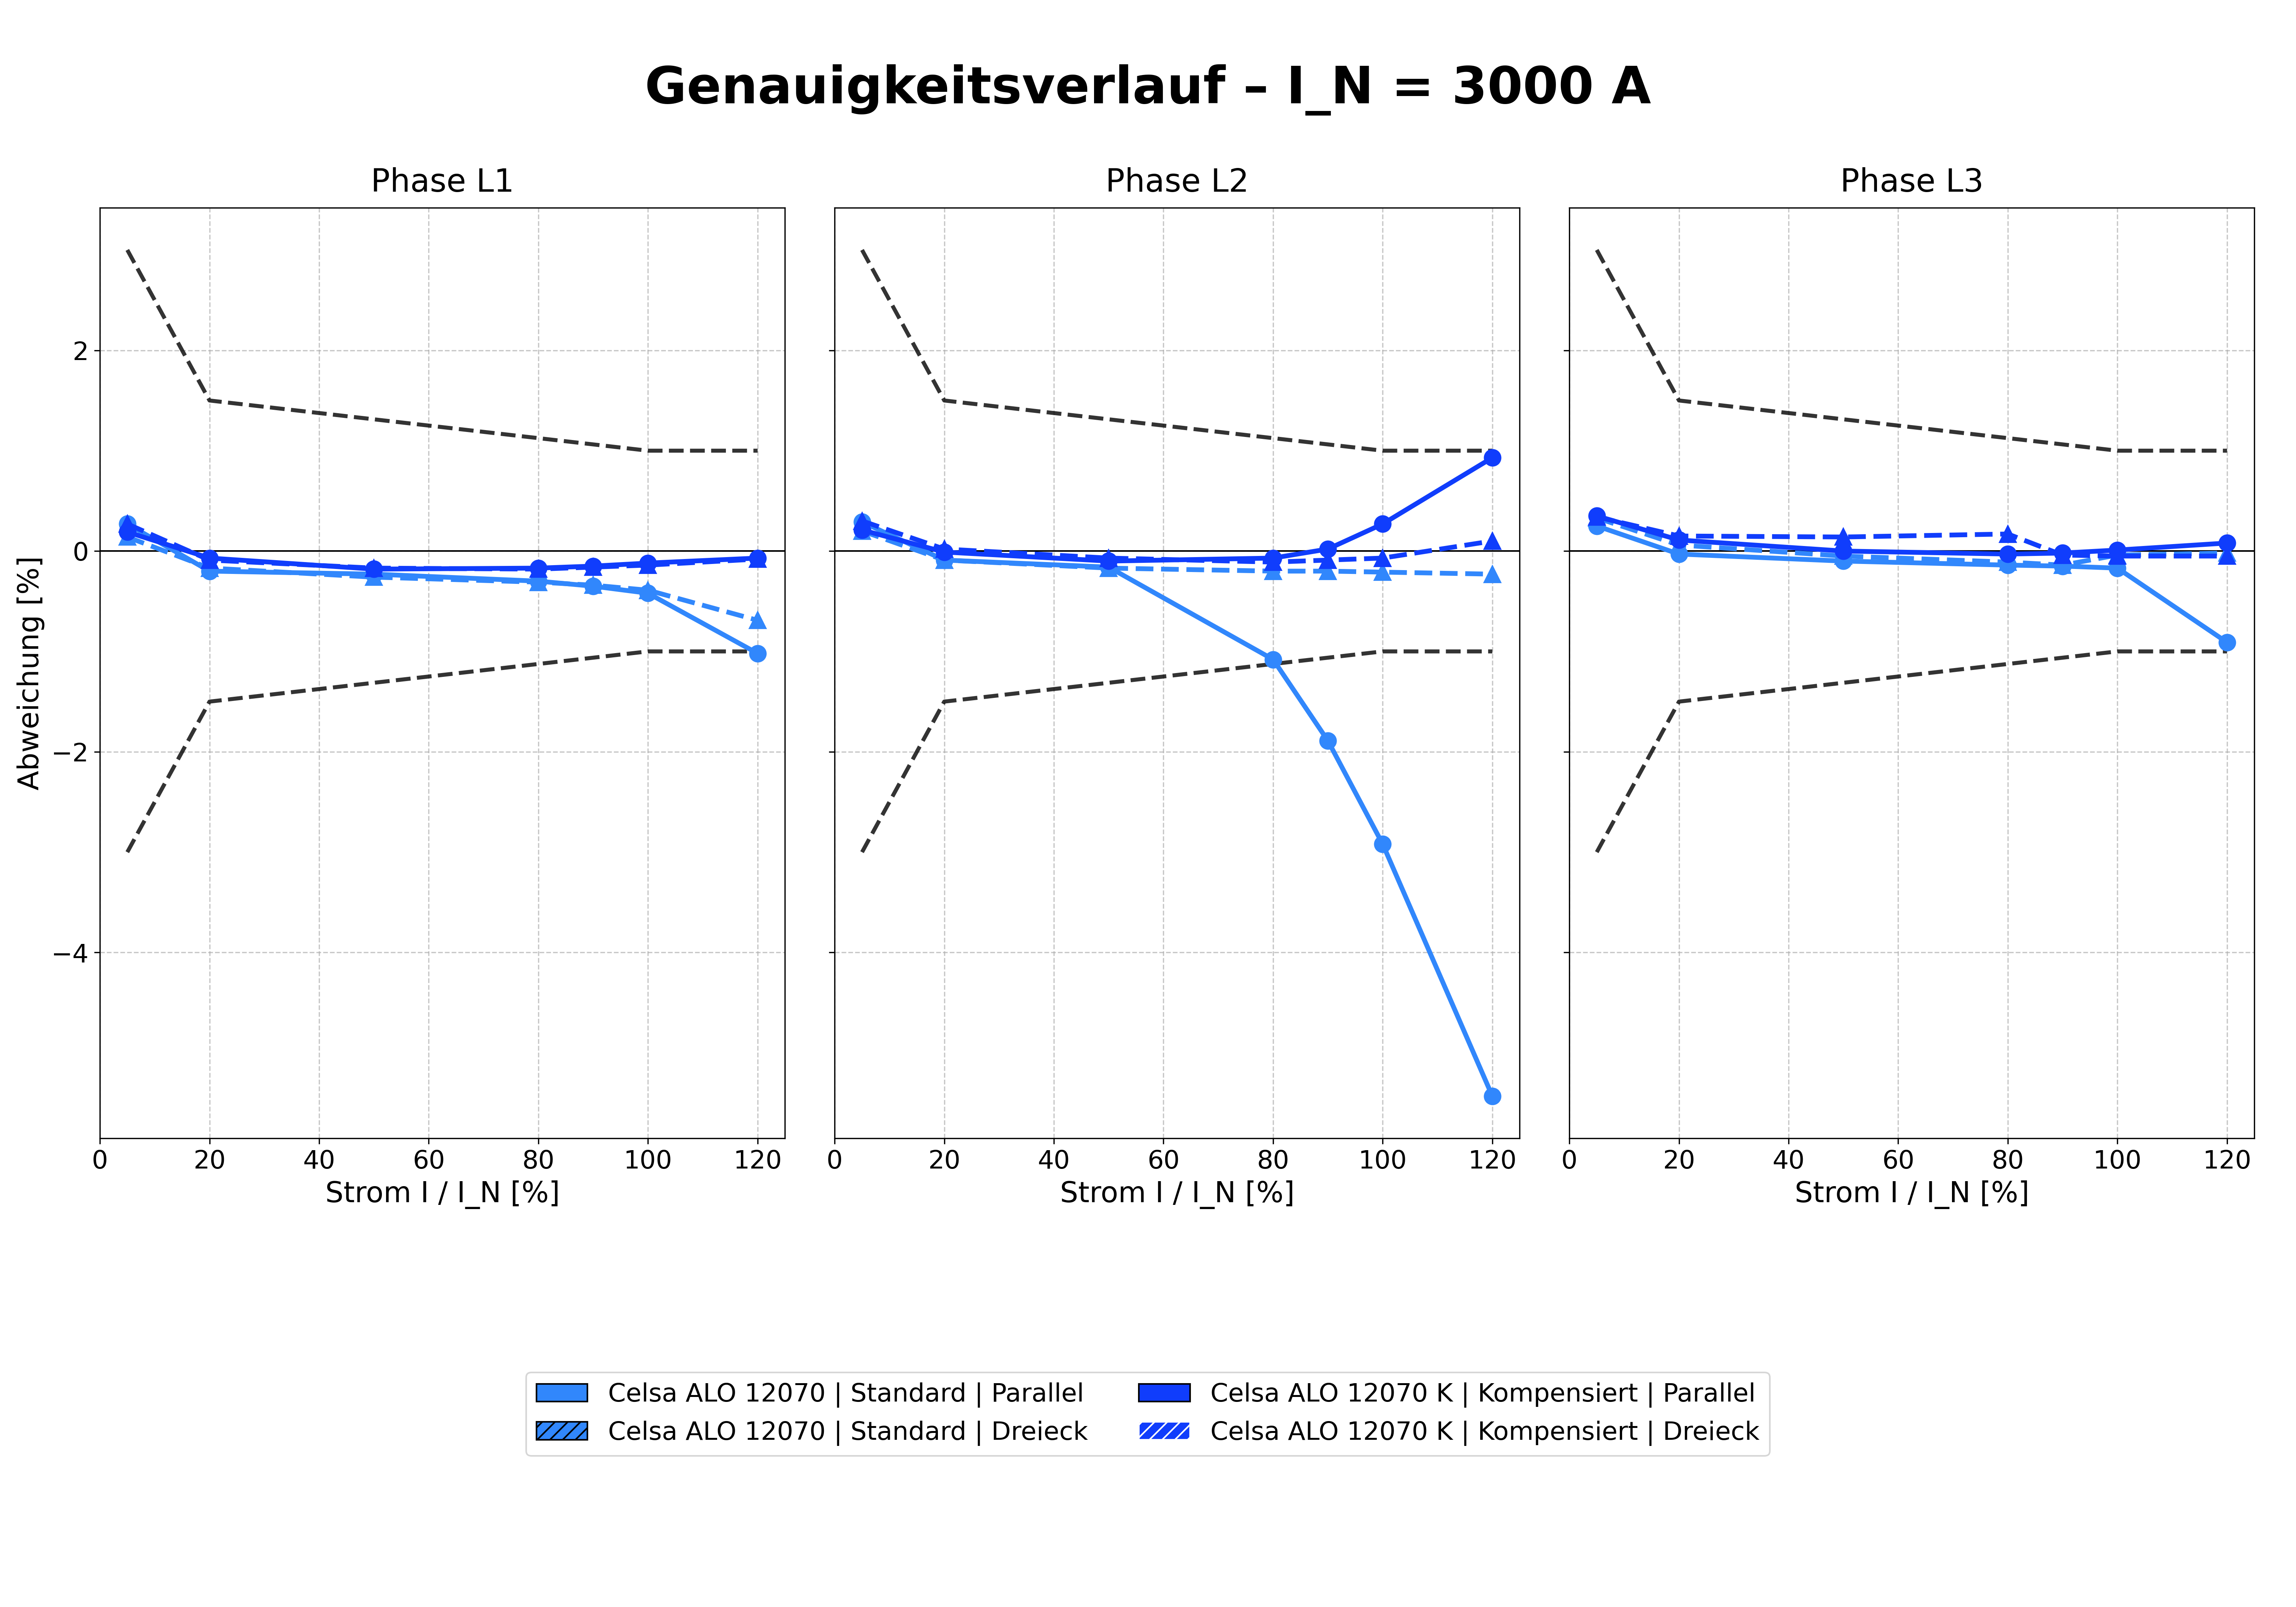
\includegraphics[width=1.0\textwidth]{03_Ressourcen/dia_neu/verlauf/mes_3000A_verlauf.png}
    \caption{Fehlerverläufe der Wandlertypen bei \SI{3000}{A} in Abhängigkeit von Leitergeometrie und Wandlerkonzept}
    \label{dia:3000A_zusammenfassung}
\end{diagram}

Zur Verdichtung der Beobachtungen über den gesamten Lastbereich ist in Abbildung~\ref{dia:3000A_bereichsanalyse} eine Bereichsanalyse des mittleren absoluten Fehlers dargestellt. Für den Standardwandler \textit{Celsa~ALO~12070} zeigt sich insbesondere in Parallelanordnung eine deutliche Verschlechterung im Hochlastbereich: Der mittlere Fehler steigt von \num{0,18}\,\% (Niederstrom) über \num{0,82}\,\% (Nennstrom) auf \num{2,45}\,\% bei \SI{120}{\percent}. In der Dreiecksanordnung bleibt der Fehler dagegen auch in Überlast mit \num{0,31}\,\% vergleichsweise niedrig. Beim kompensierten \textit{Celsa~ALO~12070~K} liegen die Fehlerwerte in beiden Geometrien über alle Lastbereiche unter \num{0,31}\,\%, was die erhöhte Sättigungsfestigkeit dieses Konzepts bestätigt.

\begin{diagram}[H]
    \centering
    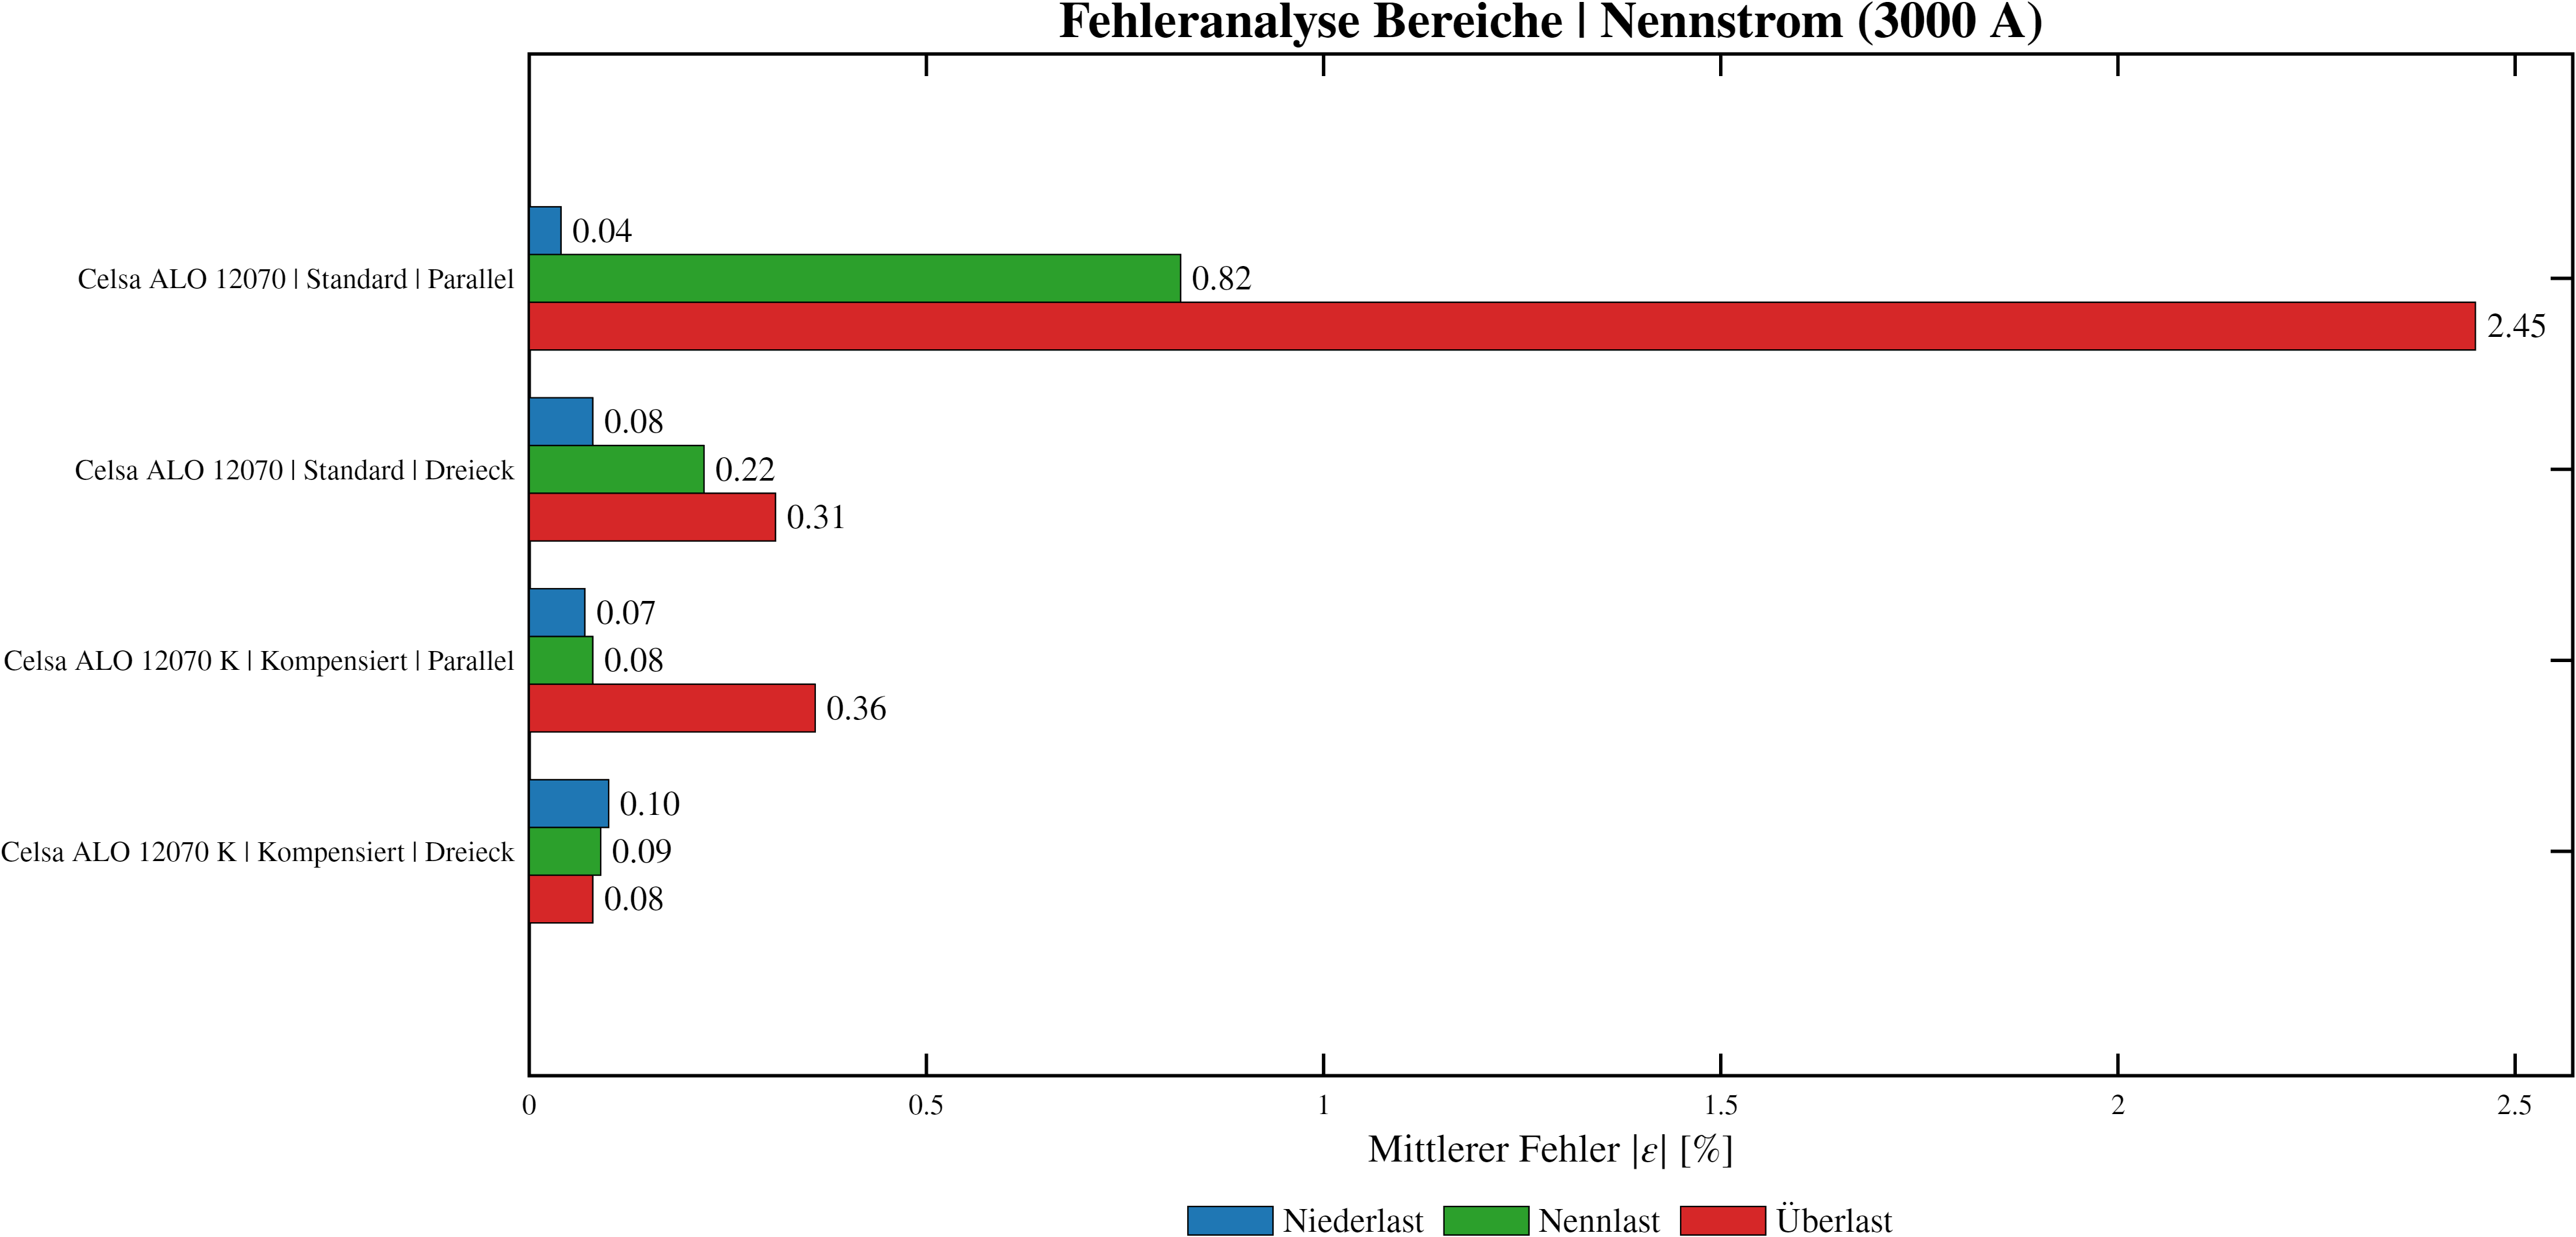
\includegraphics[width=1.0\textwidth]{03_Ressourcen/dia_neu/bereichs_analyse/mes_3000A_bereichs_analyse.png}
    \caption{Fehleranalyse nach Lastbereich bei \SI{3000}{A}: mittlerer absoluter Fehler im Niederstrom-, Nennstrom- und Überlastbereich (Standard vs.\ kompensiert; Vergleich Parallel- und Dreiecksanordnung)}
    \label{dia:3000A_bereichsanalyse}
\end{diagram}


\paragraph{Analyse der Bürdenabhängigkeit}

Da der Standardwandler in der Parallelanordnung deutliche Sättigungserscheinungen zeigt, wird ergänzend der Einfluss der Bürde untersucht. Dafür werden drei Bürdenkonfigurationen betrachtet. Tabelle~\ref{tab:buerden_konfigurationen_3000A} fasst die Referenzlast, die Minimallast sowie eine asymmetrische Last zusammen, bei der ausschließlich Phase L2 entlastet wird.

\begin{table}[H]
    \centering
    \caption{Übersicht der untersuchten Bürdenkonfigurationen bei \SI{3000}{A}}
    \label{tab:buerden_konfigurationen_3000A}
    \small
    \begin{tabular}{l S[table-format=2.2] S[table-format=2.2] S[table-format=2.2] l}
        \toprule
                           & \multicolumn{3}{c}{Bürdenwiderstand \gls{sym:RB} [\unit{\ohm}]} &                                                        \\
        \cmidrule(lr){2-4}
        {Konfiguration}    & {L1}                                                            & {L2}  & {L3}  & {Ziel der Untersuchung}                \\
        \midrule
        Referenzlast       & 10.80                                                           & 10.80 & 10.80 & Basisvergleich Geometrieeinfluss       \\
        Minimallast        & 0.00                                                            & 0.00  & 0.00  & Bestimmung maximaler Sättigungsgrenze  \\
        Asymmetrische Last & 10.80                                                           & 0.00  & 10.80 & Selektive Entlastung des Mittelleiters \\
        \bottomrule
    \end{tabular}
\end{table}

Abbildung~\ref{dia:3000A_buerde_verlauf} zeigt die Fehlerkurven des Standardwandlers \textit{Celsa~ALO~12070} in der Parallelanordnung für diese Bürdenvarianten. Für die Außenleiter L1 und L3 ergibt sich über weite Bereiche nur eine geringe Bürdenabhängigkeit. Die Abweichungen bleiben im Niederstrom- und Nennstrombereich klein und ändern sich zwischen den Varianten nur schwach. Deutlich ausgeprägter ist der Effekt bei Phase L2. Hier treten die dominierenden Abweichungen im oberen Lastbereich auf, was mit einer beginnenden magnetischen Sättigung konsistent ist.

\begin{diagram}[H]
    \centering
    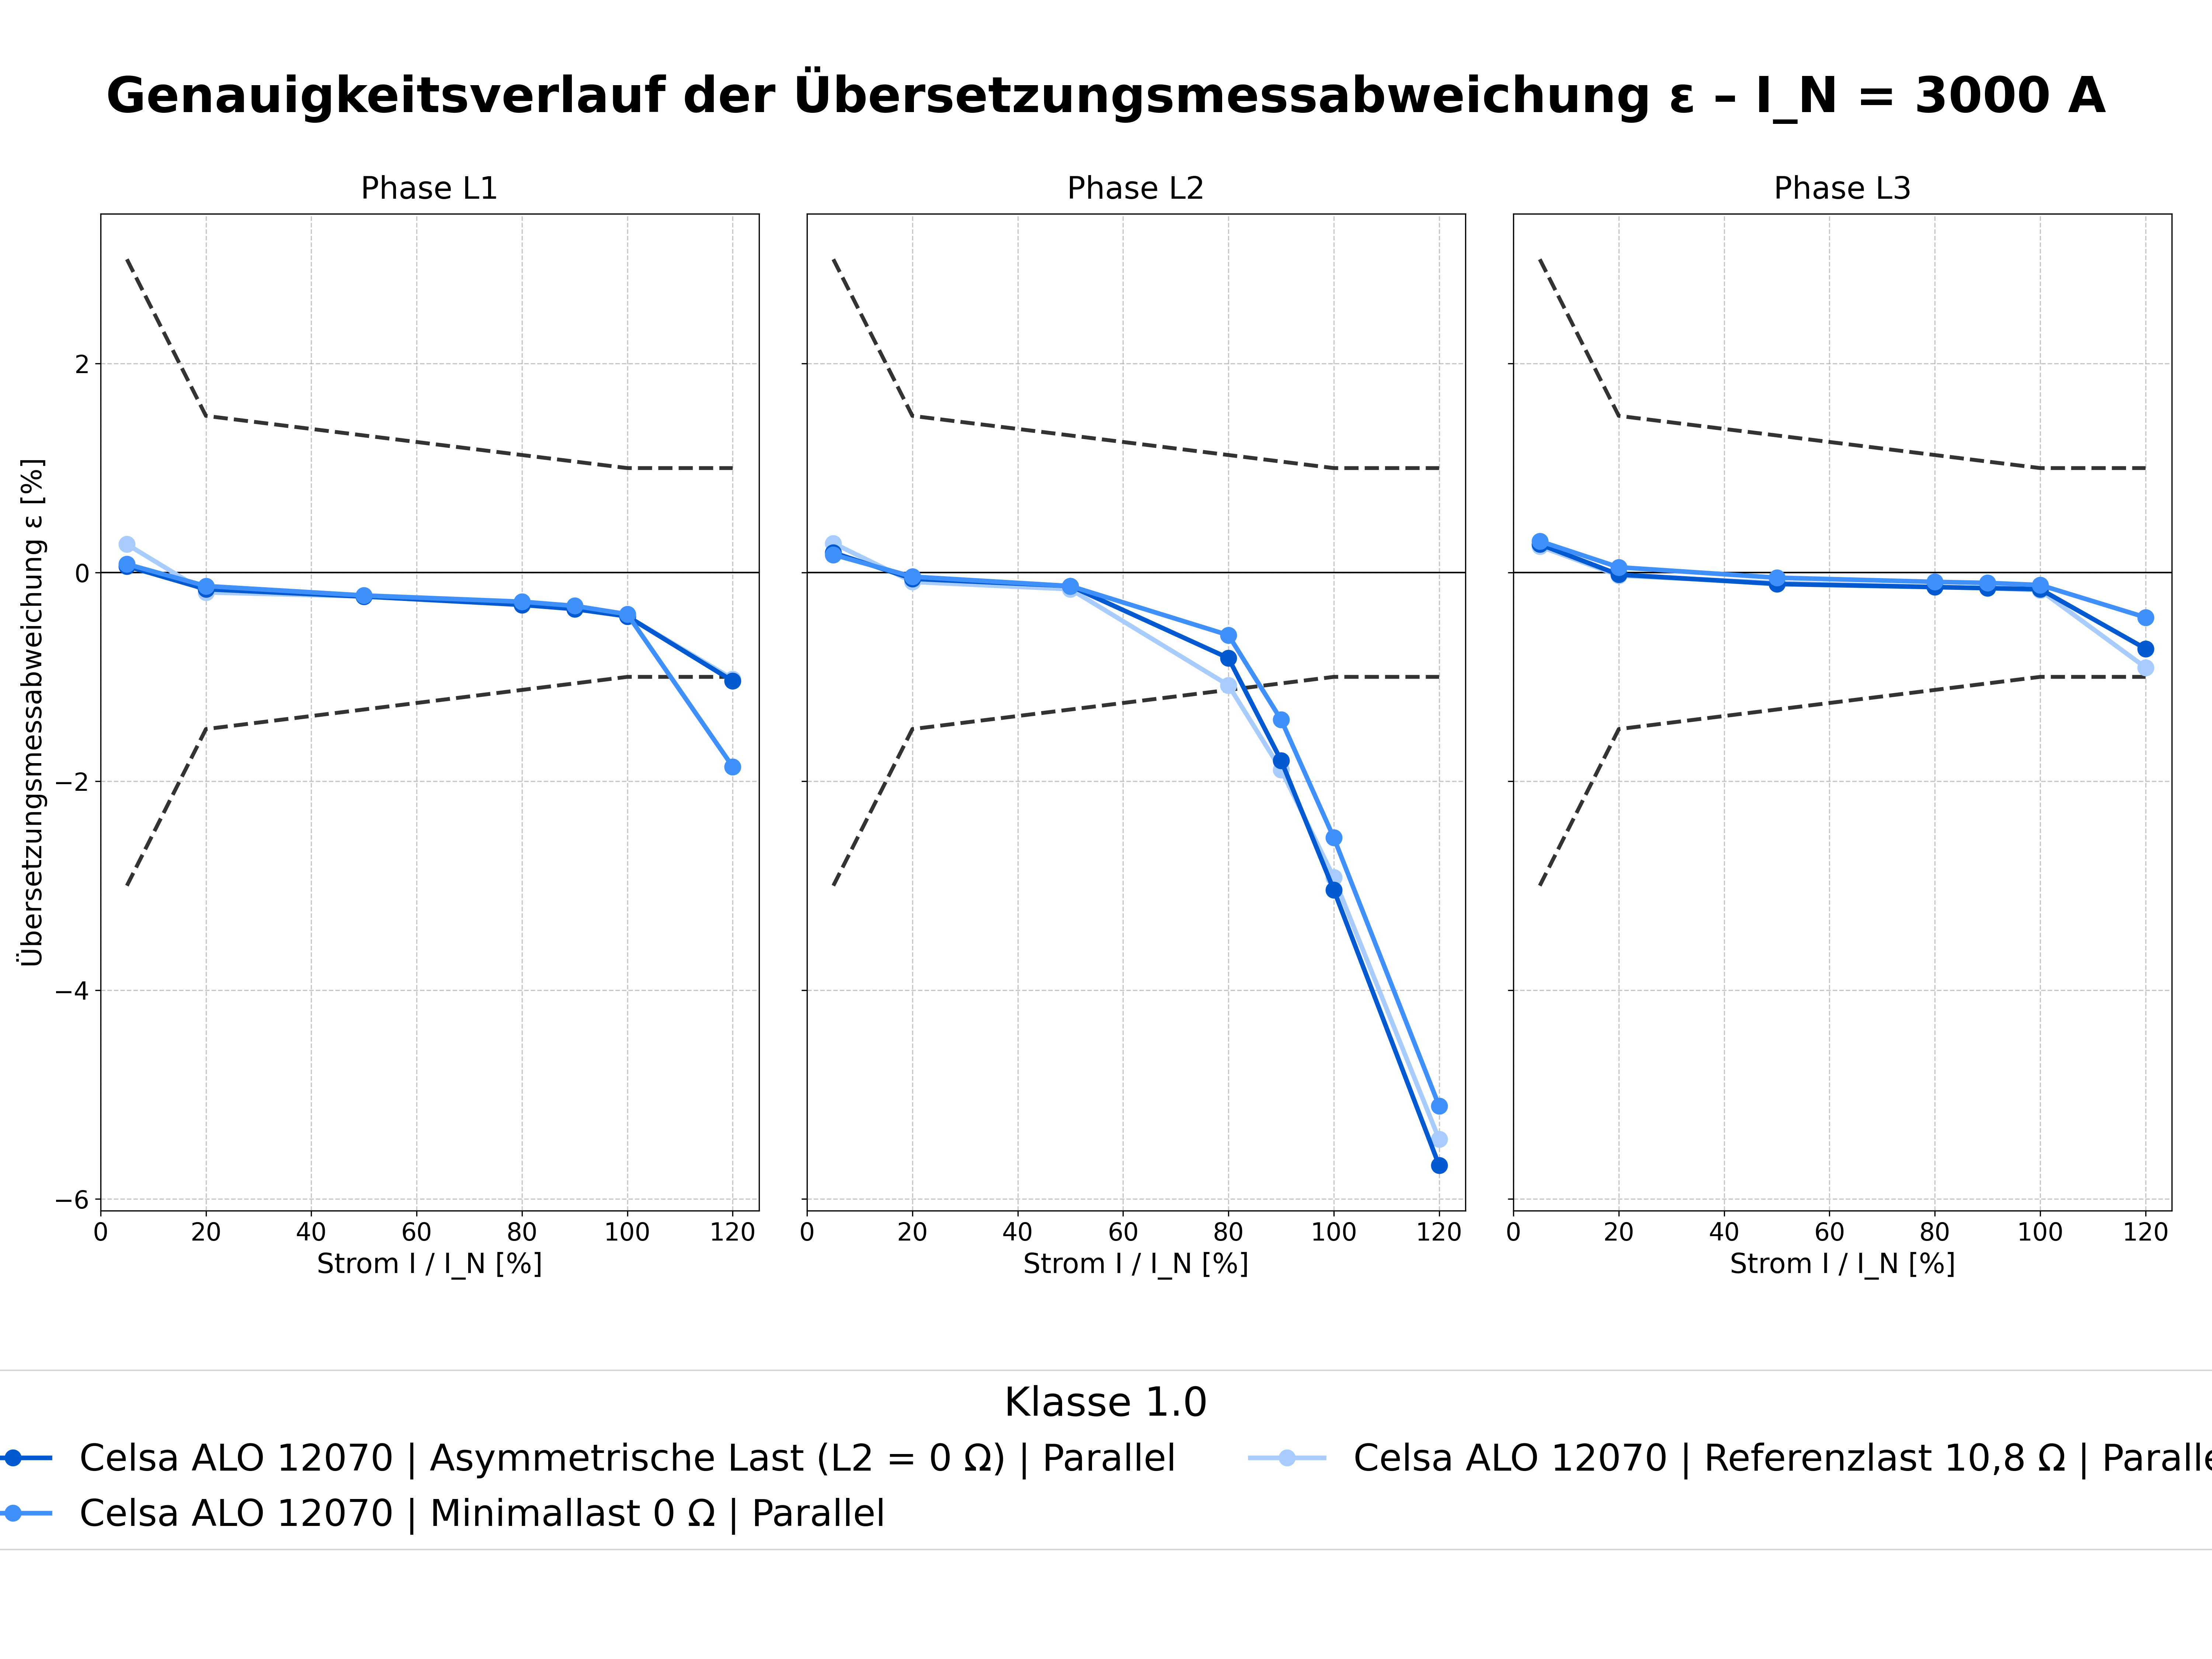
\includegraphics[width=1.0\textwidth]{03_Ressourcen/dia_neu/verlauf/mes_3000A_buerde_verlauf.png}
    \caption{Fehlerkurven des Standardwandlers bei \SI{3000}{A} in Parallelanordnung bei variabler Bürde \gls{sym:RB}}
    \label{dia:3000A_buerde_verlauf}
\end{diagram}

Der Vergleich der Referenzlast mit der asymmetrischen Last zeigt bei Phase L2 ein nahezu identisches Verhalten. Bei \SI{100}{\percent} des Nennstroms \gls{sym:In} liegt die asymmetrische Last bei \num{-3,00}\,\%, während die Referenzlast \num{-2,90}\,\% erreicht. Auch bei \SI{120}{\percent} bleiben die Werte vergleichbar. Die asymmetrische Last erreicht \num{-5,70}\,\% und die Referenzlast \num{-5,40}\,\%. Die Entlastung ausschließlich von L2 führt damit in dieser Messreihe nicht zu einer deutlichen Reduktion der Abweichung im Hochlastbereich.

Die Minimallast zeigt für Phase L2 die geringsten Abweichungen im Bereich bis etwa \SI{90}{\percent}. Bei \SI{80}{\percent} liegt der Fehler bei \num{-0,60}\,\%, während die Referenzlast bei \num{-1,10}\,\% liegt. Im Bereich des Nennstroms und darüber bleibt jedoch auch bei Minimallast eine deutliche Abweichung bestehen. Bei \SI{100}{\percent} ergibt sich \num{-2,50}\,\%, womit die Genauigkeitsklasse \num{1} weiterhin nicht eingehalten wird.

\begin{diagram}[H]
    \centering
    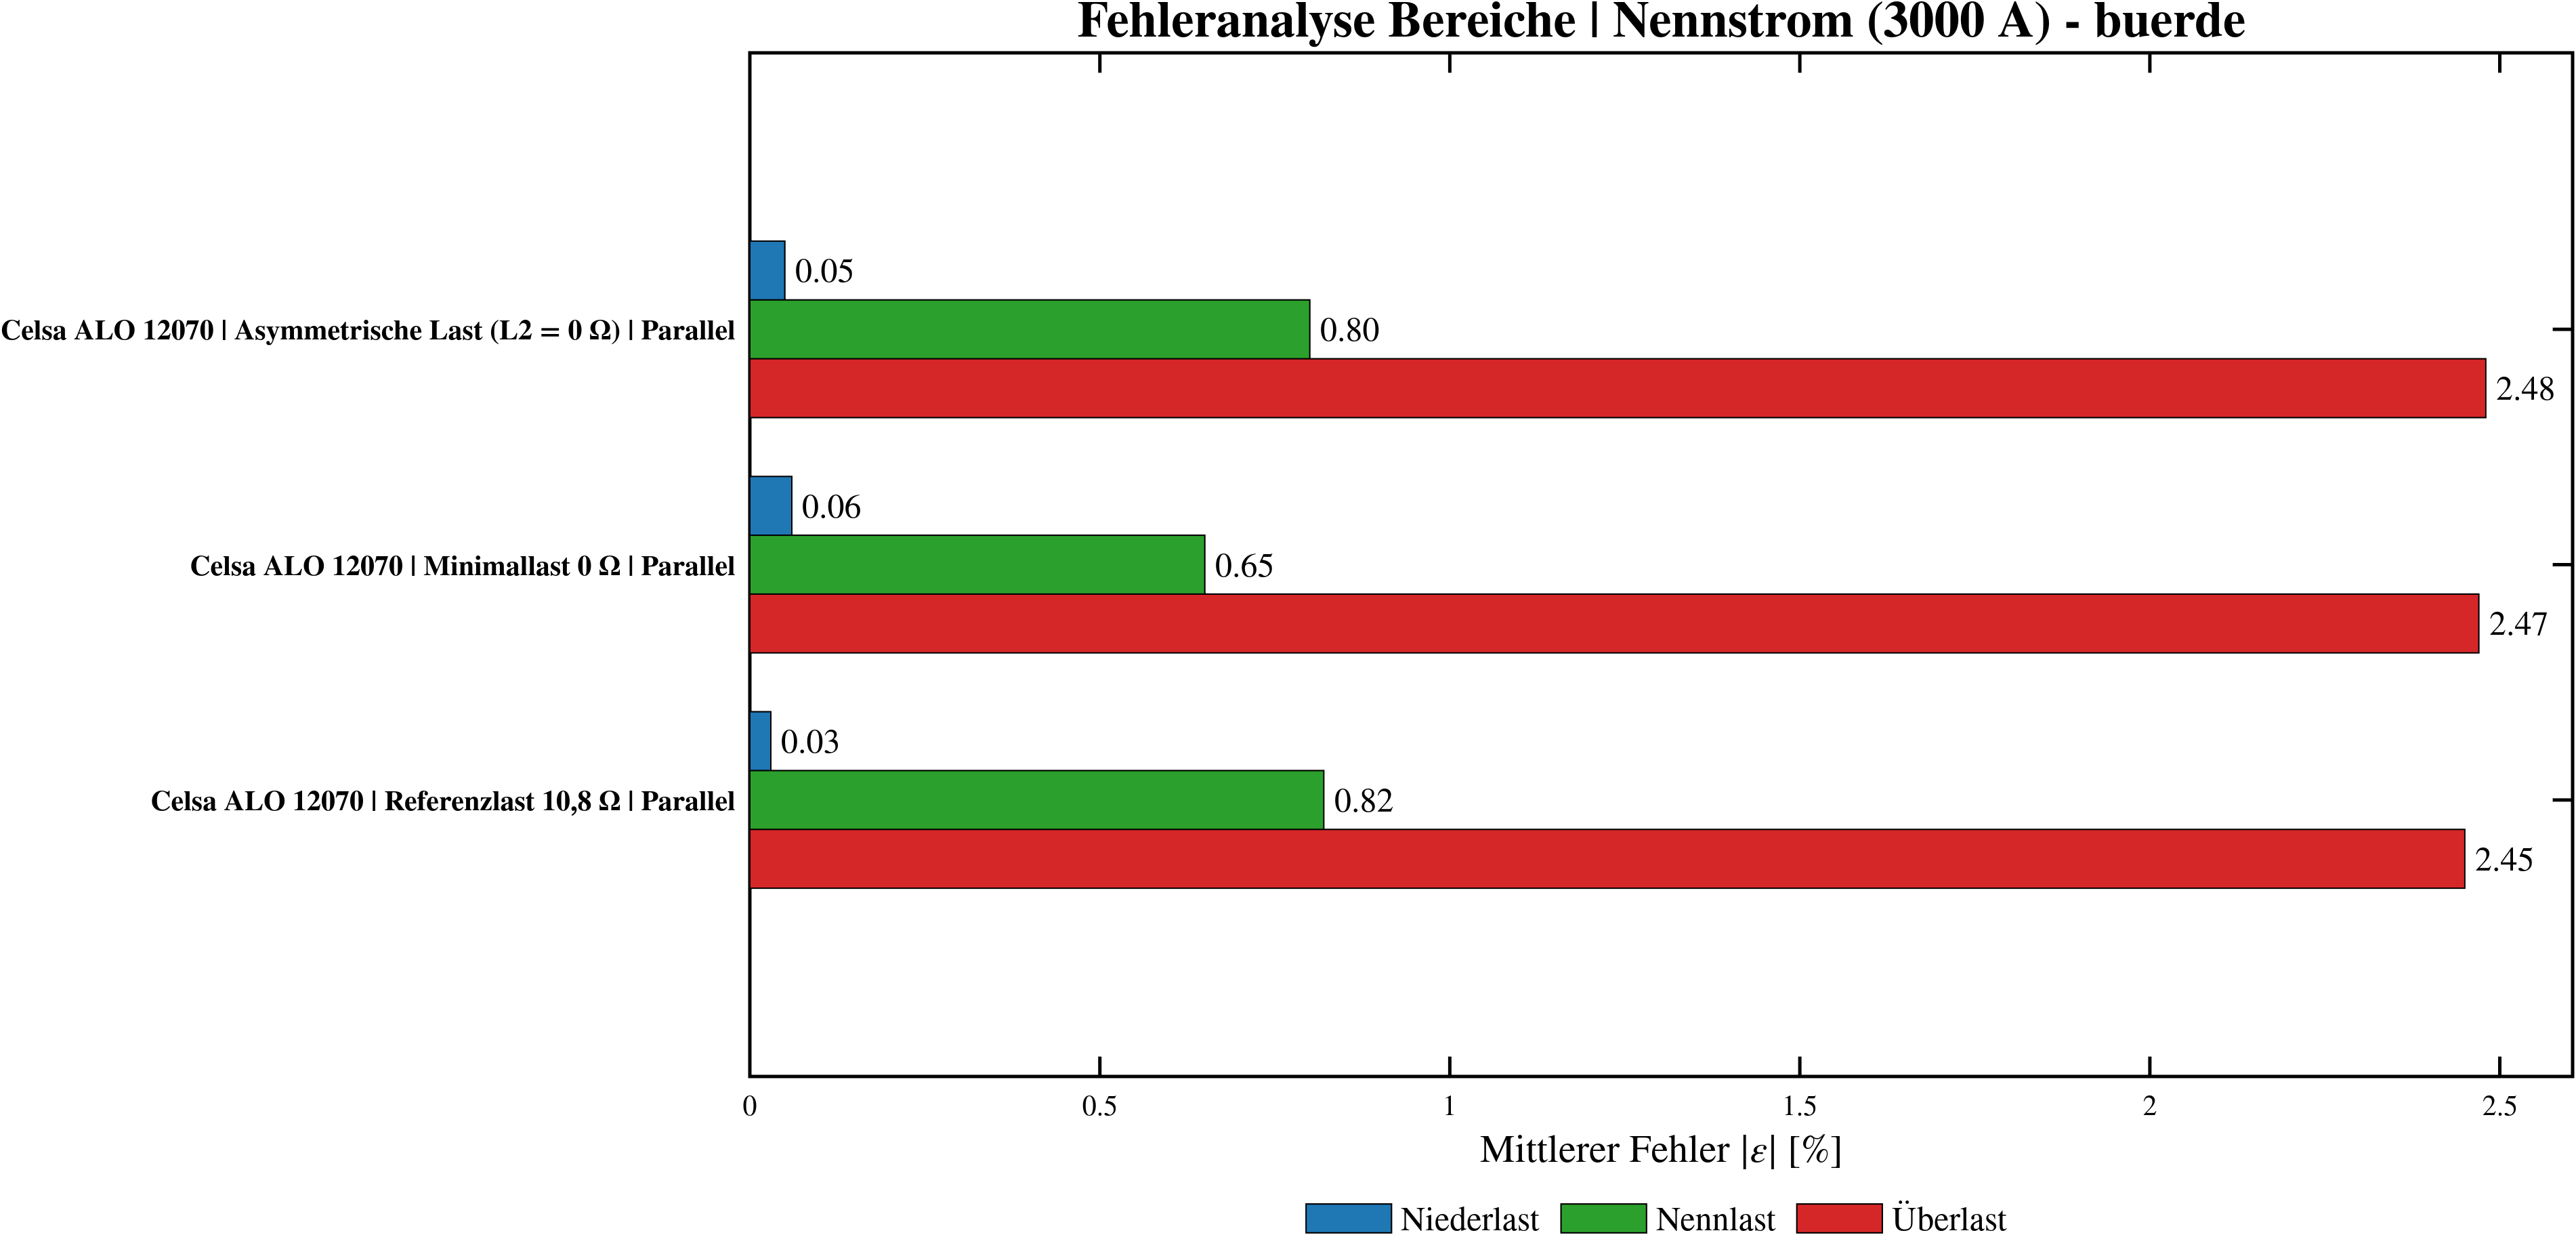
\includegraphics[width=1.0\textwidth]{03_Ressourcen/dia_neu/bereichs_analyse/mes_3000A_buerde_bereichs_analyse.png}
    \caption{Fehleranalyse nach Lastbereich bei \SI{3000}{A} in Parallelanordnung: Einfluss der Bürdenkonfiguration auf den mittleren absoluten Fehler (von unten nach oben: Referenzlast, Minimallast, asymmetrische Last)}
    \label{dia:3000A_bereichsanalyse_buerde}
\end{diagram}

Abbildung~\ref{dia:3000A_bereichsanalyse_buerde} fasst die drei Bürdenvarianten aus Abbildung~\ref{dia:3000A_buerde_verlauf} über die Lastbereiche zusammen. Die Variation wirkt sich im Mittel vor allem im Nennstrombereich aus: Die Minimallast reduziert den mittleren Fehler von \num{0,82}\,\% (Referenzlast) auf \num{0,65}\,\%, während die asymmetrische Last mit \num{0,80}\,\% nahe am Referenzfall bleibt. Im Überlastpunkt bleiben die Unterschiede hingegen gering (\num{2,45}--\num{2,48}\,\%), was die zuvor beobachtete Dominanz der Sättigungseffekte im Standardwandler bestätigt. Insgesamt wird damit sichtbar, dass eine Bürdenreduktion zwar messbar ist, der Einfluss von Leitergeometrie und Wandlerkonzept jedoch deutlich stärker wirkt.
\subsubsection{Skalierung der Geometrieeffekte bei \SI{4000}{A}}
\label{sec:analyse_messreihe_4000A}

Für diese Messreihe wurde der Phasenmittenabstand gemäß Tabelle~\ref{tab:schienen_konfiguration} auf den für diese Stromstärke üblichen Wert vergrößert. Mit der Steigerung des Nennstroms \gls{sym:In} auf \SI{4000}{A} rückt die Reproduzierbarkeit der geometrischen Einflüsse bei gleicher Wandlerbauform in den Vordergrund. Betrachtet werden erneut die Typen der Reihe \textit{Celsa~ALO~12070} in Standardausführung sowie in der kompensierten Variante \textit{Celsa~ALO~12070~K}. Die Ergebnisse dienen dazu, das Verhalten der Wandler bei weiter steigender Sättigung ohne den Einfluss variabler Bürdenwiderstände zu verifizieren.



Abbildung~\ref{dia:4000A_zusammenfassung} skizziert einen Verlauf, der qualitativ stark den Beobachtungen aus Abschnitt \ref{sec:analyse_messreihe_3000A} ähnelt. Sowohl in der Parallelanordnung als auch in der Dreieckskonfiguration stößt der Standardwandler \textit{Celsa~ALO~12070} hier an seine physikalischen Leistungsgrenzen, wenngleich zu unterschiedlichen Zeitpunkten.

\begin{diagram}[H]
    \centering
    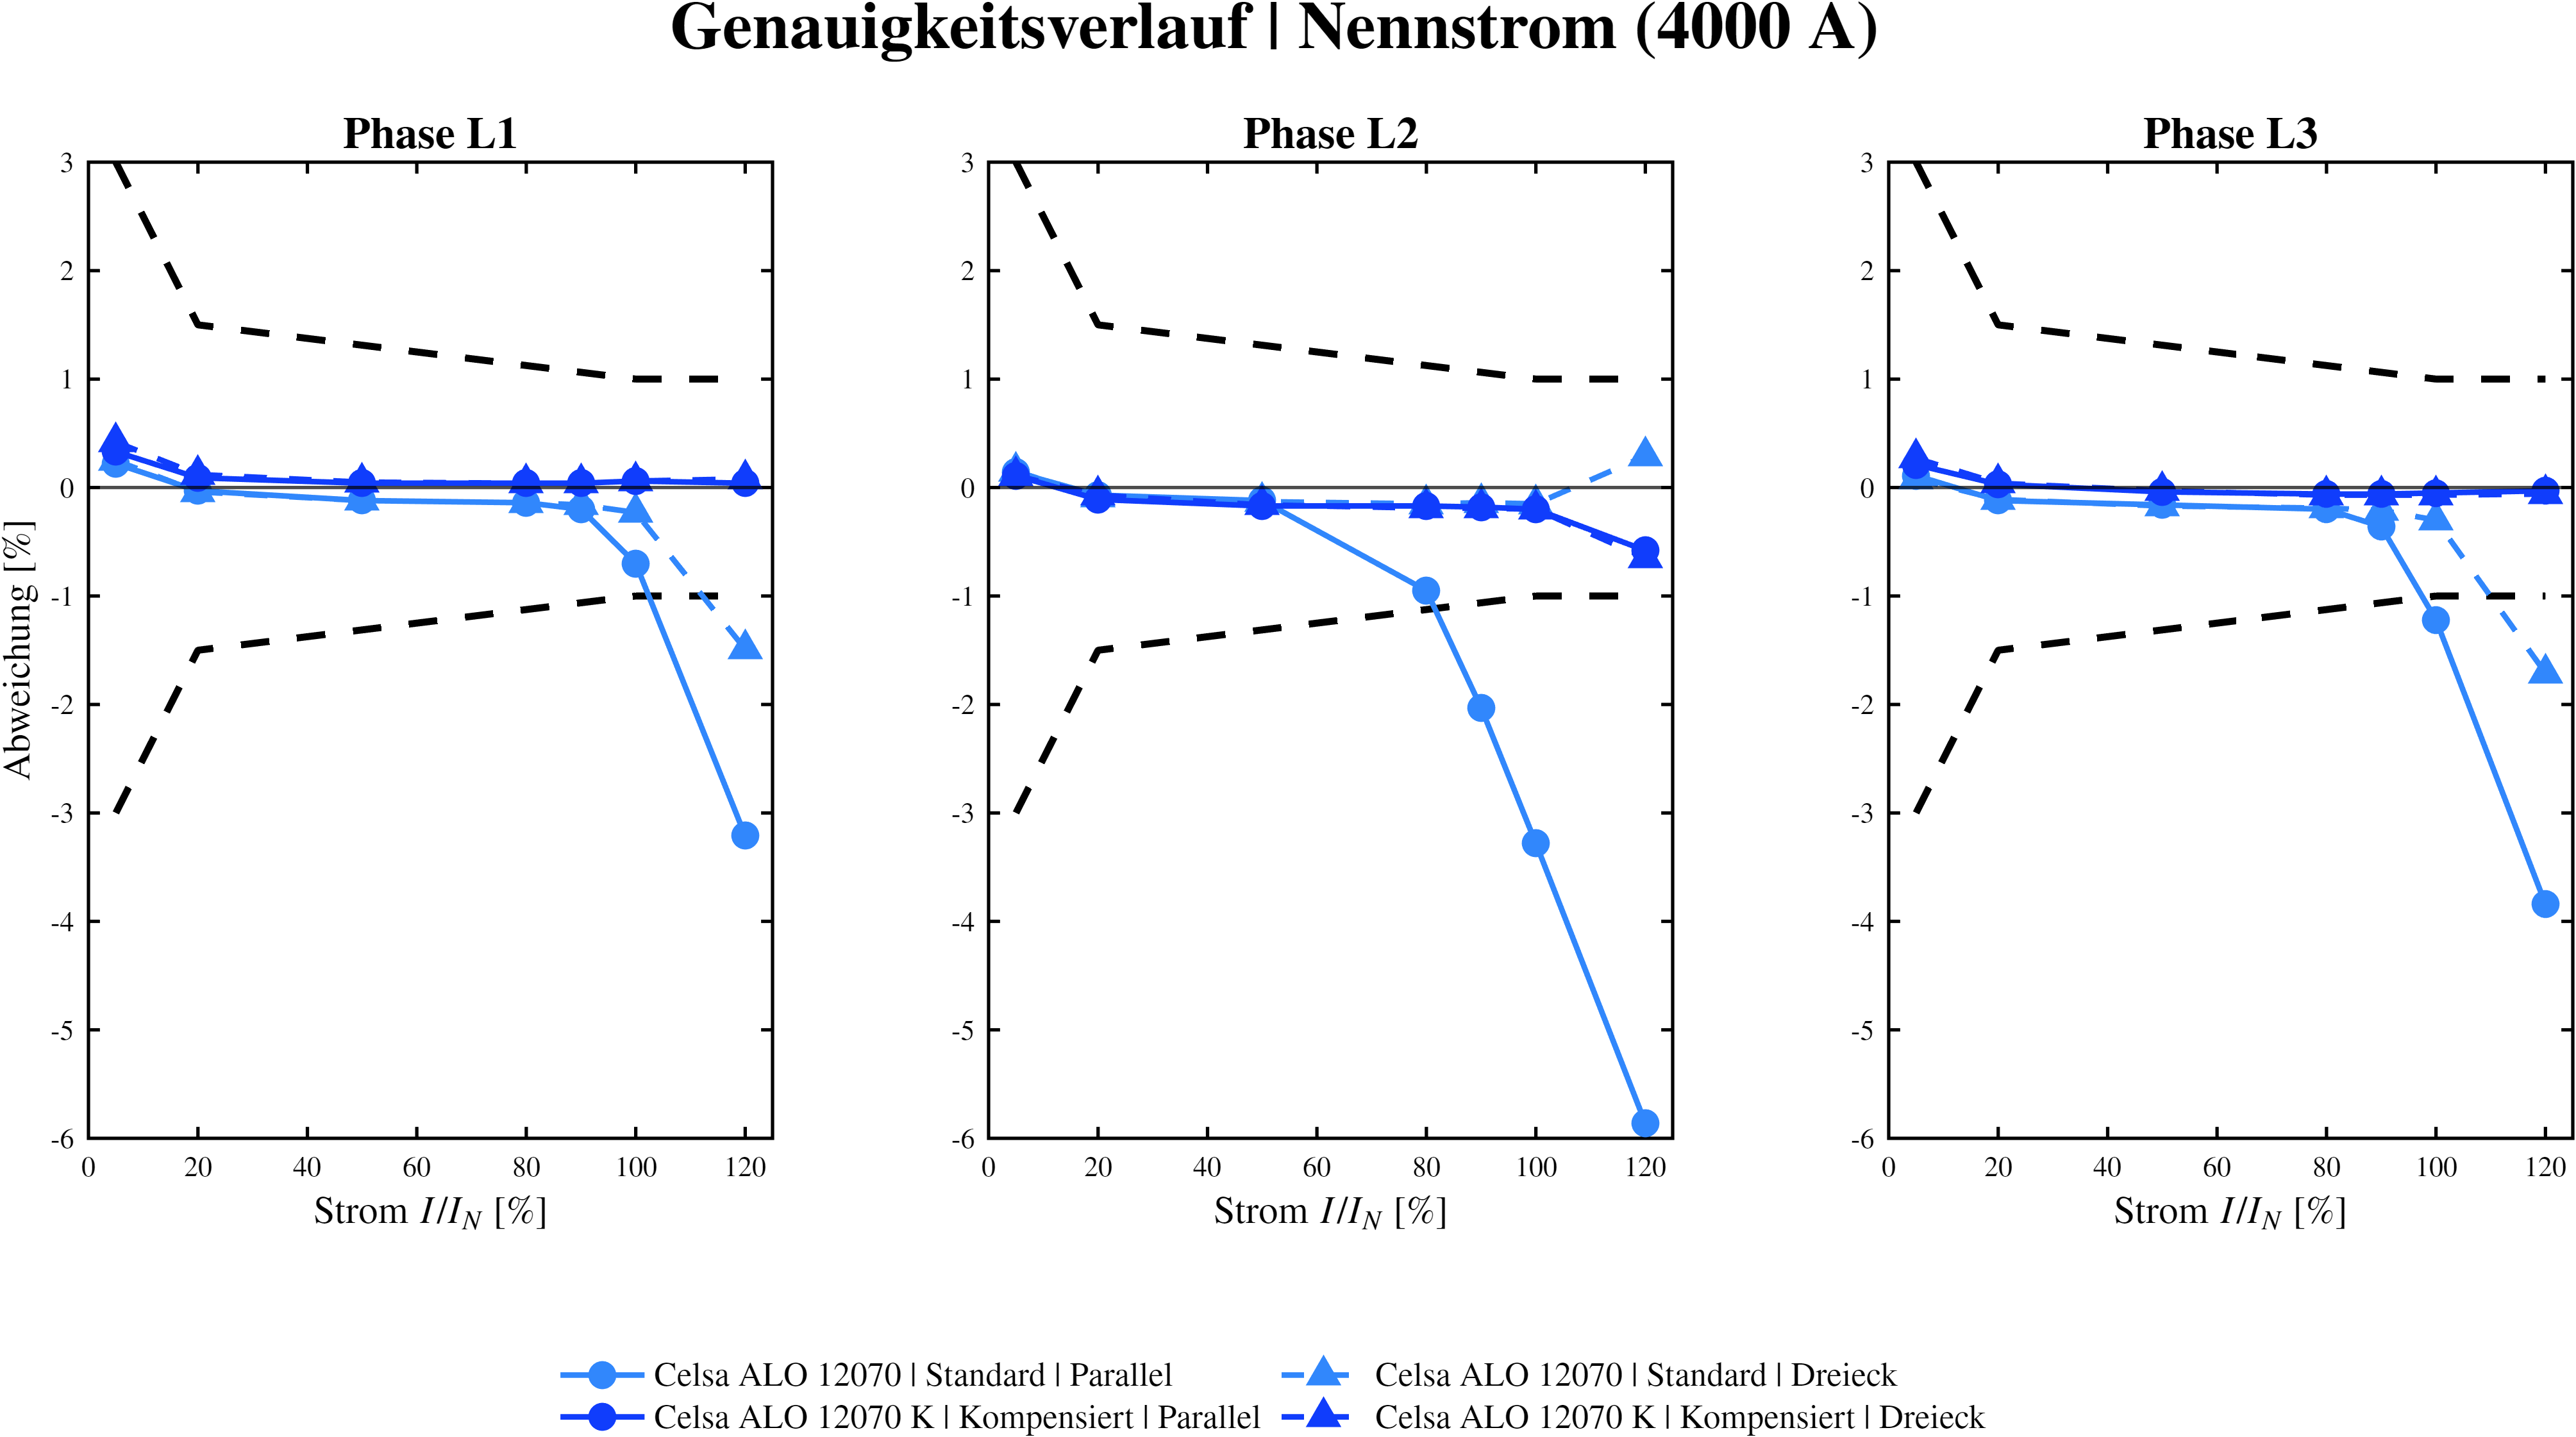
\includegraphics[width=1.0\textwidth]{03_Ressourcen/dia_neu/verlauf/mes_4000A_verlauf.png}
    \caption{Übersetzungsmessabweichung \gls{sym:epsilon} bei \SI{4000}{A}: Vergleich von Parallel- und Dreiecksanordnung (Phasen L1--L3)}
    \label{dia:4000A_zusammenfassung}
\end{diagram}

Besonders augenfällig wird dies in der Parallelanordnung. Wie die Werte in Tabelle~\ref{tab:messergebnisse_celsa12070_4000A_alle} im Anhang belegen, bricht die Genauigkeit ab \SI{80}{\percent} des Nennstroms \gls{sym:In} drastisch ein. Bei \SI{3200}{A} weist der mittlere Leiter L2 bereits eine Übersetzungsmessabweichung \gls{sym:epsilon} von \num{-0,90}\,\% auf und verlässt bei weiterer Lasterhöhung den Toleranzbereich der Genauigkeitsklasse \num{1}. Bei Nennstrom (\SI{4000}{A}) liegt der Fehler bei \num{-3,30}\,\%.

Dieser Einbruch bei etwa \SI{3200}{A} korreliert signifikant mit den Sättigungseffekten der \SI{3000}{A}-Messreihe, was darauf hindeutet, dass die physikalische Sättigungsgrenze des Eisenkerns in der Parallelgeometrie in diesem Lastbereich liegt. Dieses Verhalten spiegelt die Problematik wider, welche bereits beim Typ \textit{Celsa~ALO~10030} bei \SI{2000}{A} und \SI{2500}{A} beobachtet wurde, wo die Parallelanordnung ebenfalls zu einer vorzeitigen Sättigung durch Fremdfeldeinflüsse führte.

Zur kompakten Gegenüberstellung der Geometrieeffekte über den Lastbereich zeigt Abbildung~\ref{dia:4000A_bereichsanalyse} eine Bereichsanalyse des mittleren absoluten Fehlers. Für den Standardwandler \textit{Celsa~ALO~12070} dominiert in Parallelanordnung der Hochlastbereich: Der mittlere Fehler steigt von \num{0,12}\,\% (Niederstrom) über \num{1,01}\,\% (Nennstrom) auf \num{4,30}\,\% bei \SI{120}{\percent}. Die Dreiecksanordnung reduziert den Fehler im Nennstrombereich auf \num{0,19}\,\%, erreicht jedoch in Überlast weiterhin \num{0,97}\,\%. Der kompensierte \textit{Celsa~ALO~12070~K} bleibt demgegenüber in beiden Geometrien über alle Lastbereiche unter \num{0,21}\,\%.

\begin{diagram}[H]
    \centering
    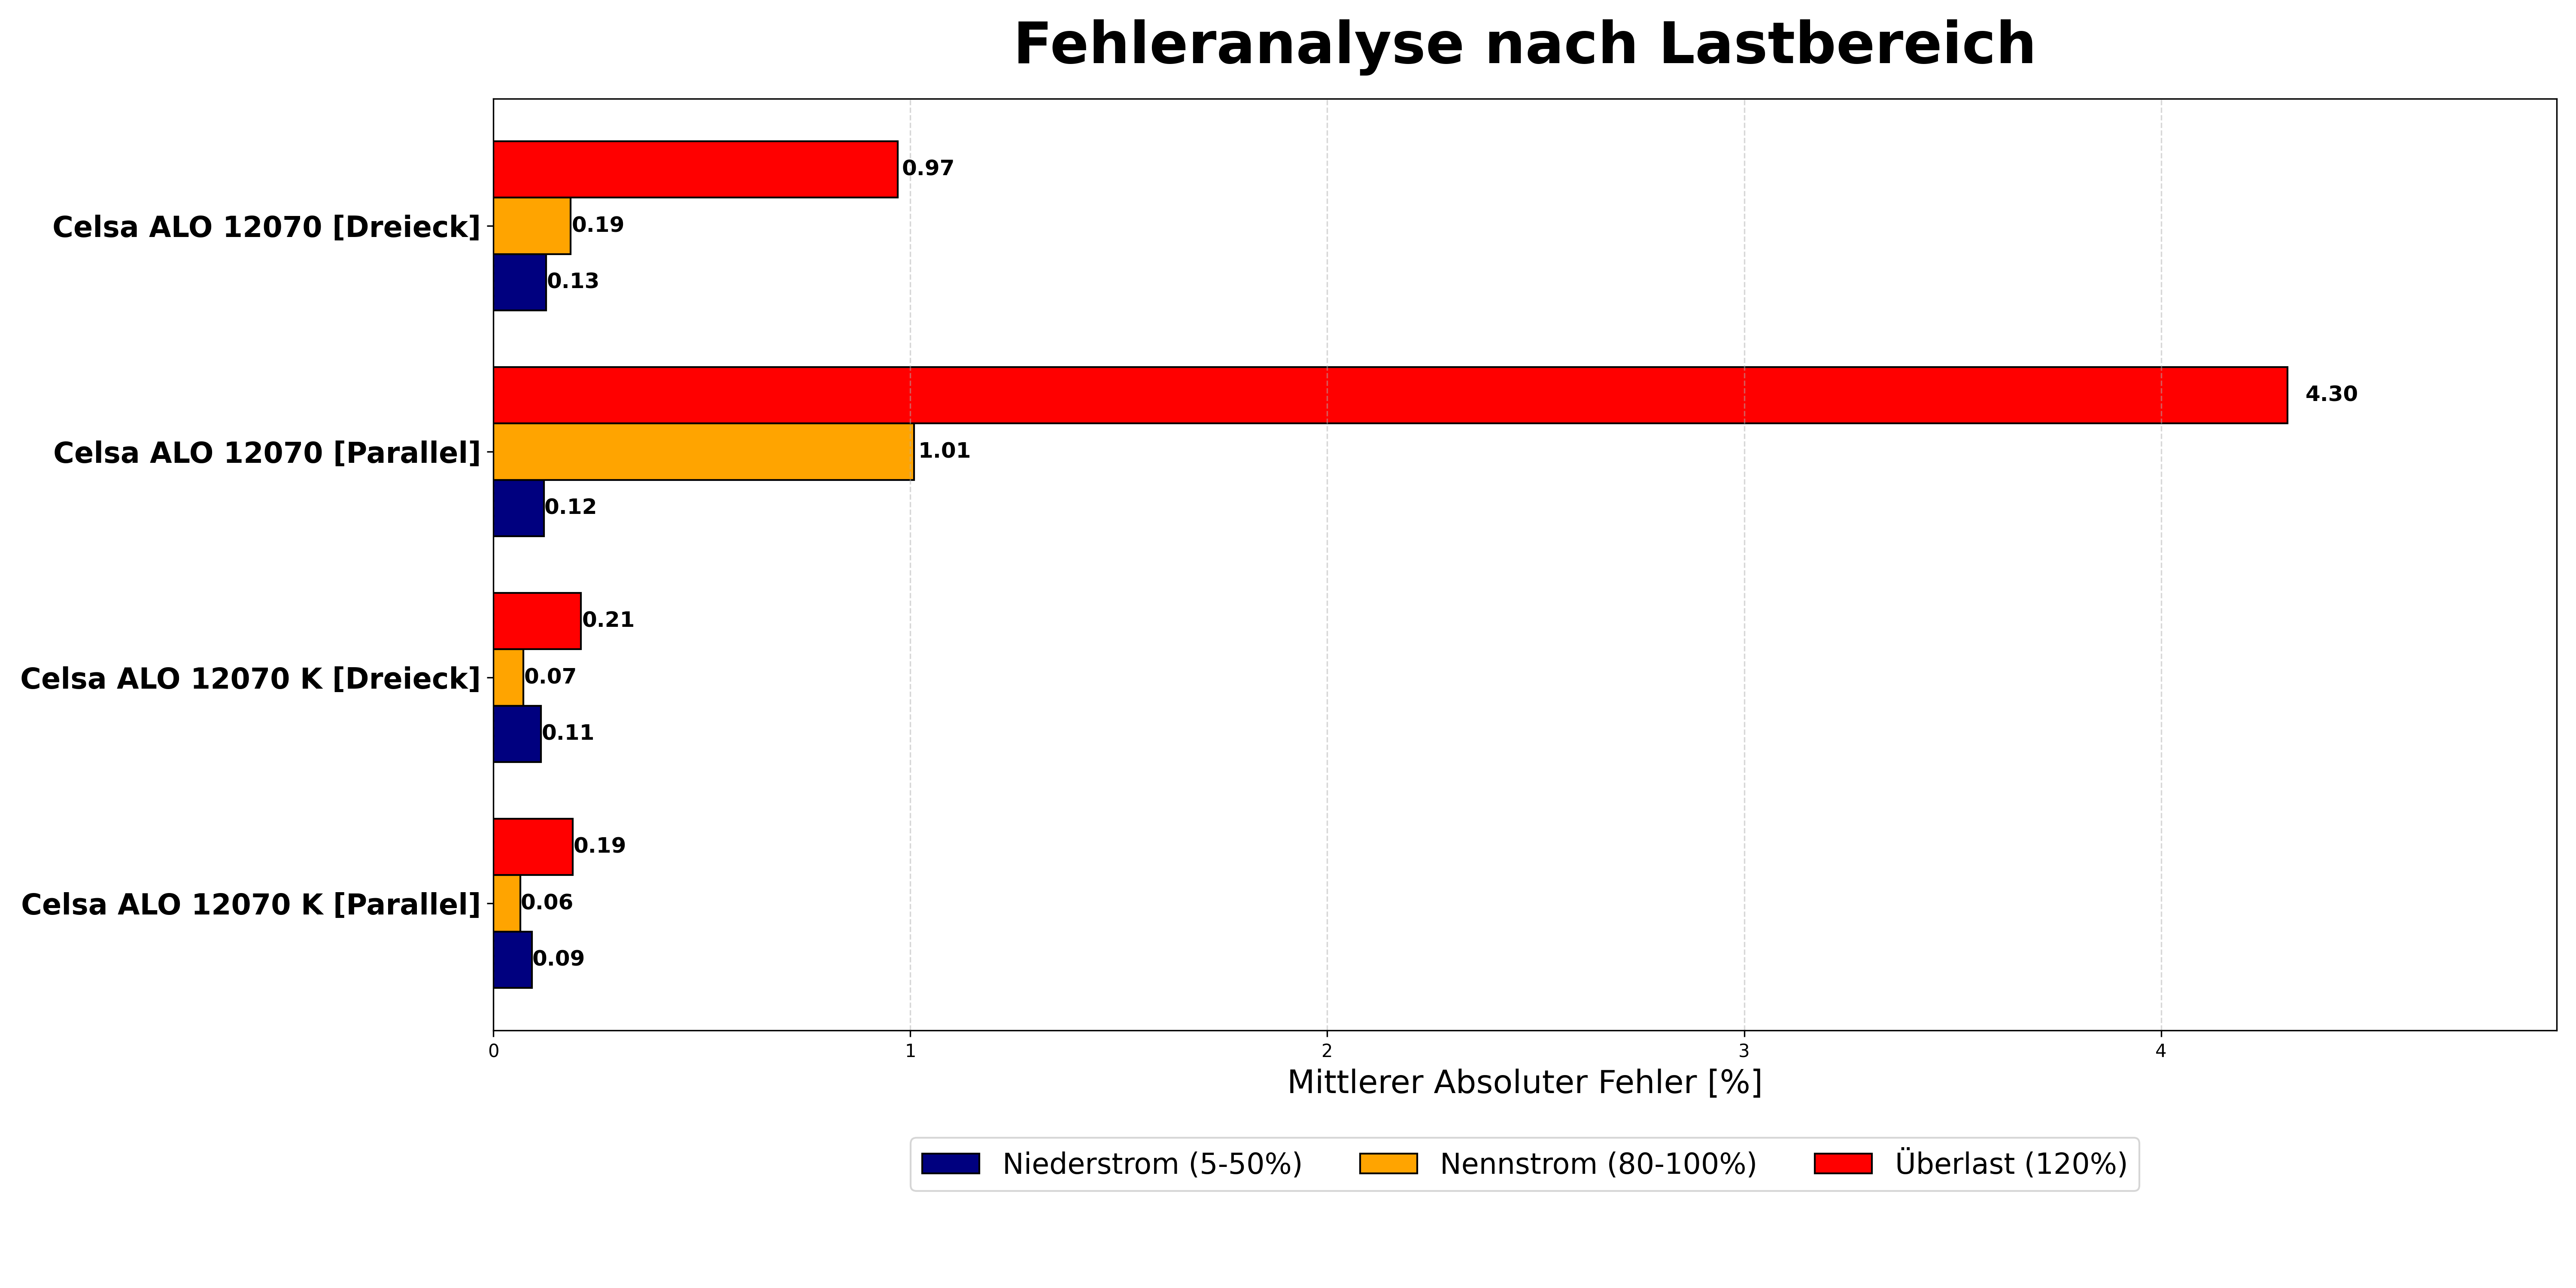
\includegraphics[width=1.0\textwidth]{03_Ressourcen/dia_neu/bereichs_analyse/mes_4000A_bereichs_analyse.png}
    \caption{Fehleranalyse nach Lastbereich bei \SI{4000}{A}: mittlerer absoluter Fehler im Niederstrom-, Nennstrom- und Überlastbereich (Standard vs.\ kompensiert; Vergleich Parallel- und Dreiecksanordnung)}
    \label{dia:4000A_bereichsanalyse}
\end{diagram}




Die Umstellung auf die Dreieckskonfiguration bewirkt bei Nennstrom eine deutliche Verbesserung. Die Abweichung \gls{sym:epsilon} der Phase L2 reduziert sich hierbei von \num{-3,30}\,\% in der Parallelanordnung auf \num{-0,15}\,\% in der Dreieckskonfiguration, womit die Genauigkeitsklasse \num{1} bei \SI{100}{\percent} Last wieder eingehalten wird. Allerdings zeigt sich im Überlastbereich bei \SI{120}{\percent}, dass auch die Dreiecksanordnung die magnetische Sättigung nicht vollständig verhindern kann, da hier die Außenleiter L1 und L3 mit \num{-1,50}\,\% beziehungsweise \num{-1,70}\,\% die normativen Klassengrenzen überschreiten.





\subsection{Ökonomische Evaluation und Technologie Ranking}
\label{sec:oekonomische_evaluation}

Die technische Bewertung der Prüflinge erfolgt über die Übersetzungsmessabweichung \gls{sym:epsilon}. Für die wirtschaftliche Einordnung wird der technische Nutzen mit den Anschaffungskosten verknüpft. Grundlage ist die Bereichsaggregation der Absolutfehler nach Gleichung~\ref{eq:fehler_bereich}. Der Vergleich zwischen Parallelanordnung und Dreiecksanordnung erfolgt über den Quotienten
\[
q_{\mathrm{Bereich}}=\frac{\bar{\varepsilon}_{\mathrm{Bereich,Dreieck}}}{\bar{\varepsilon}_{\mathrm{Bereich,Parallel}}}
\]
Werte kleiner eins bedeuten eine Verbesserung durch die Dreiecksanordnung. Die geometrische Verbesserung \(\eta_{\text{geo}}\) sowie die ökonomische Kenngröße \(\eta_{\text{eco}}\) ergeben sich daraus direkt über die bereits definierten Gleichungen~\ref{eq:eta_geo} und~\ref{eq:eta_eco}. Die Preisangaben stammen aus Tabelle~\ref{tab:wandler_spezifikationen_erweitert}.

\subsubsection{Wirtschaftlichkeit im Nennstrombereich \SI{2000}{A} bis \SI{2500}{A}}

Bei \SI{2000}{A} liegen mehrere Prüflinge im Nennbereich in ähnlichen Fehlergrößenordnungen. Der Quotient in Tabelle~\ref{tab:oeko_q_2000A} zeigt, dass die Dreiecksanordnung bei feldempfindlichen Standardwandlern im Nennbereich und im Überlastpunkt deutliche Vorteile bringt. Beim \textit{Celsa ALO 10030} sinkt der Bereichsfehler im Nennbereich stark, während der \textit{MBS ASK101.4} nur moderat profitiert. Der kompensierte \textit{Celsa ALO 8030 K} liegt in allen Bereichen nahe bei \(q\approx 1\), wodurch der zusätzliche konstruktive Aufwand die Geometrieeffekte weitgehend entkoppelt. Beim \glsentryshort{ffp} Wandler \textit{Redur 13A1030.3ffp} ist \(q\) im Nennbereich und im Überlastpunkt größer als eins, was die in Abschnitt~\ref{sec:anhang_2000A} sichtbare Empfindlichkeit der Dreiecksanordnung gegenüber der ungeschirmten Rückseite stützt.

Bei \SI{2500}{A} verschiebt sich das Bild. Der Standardwandler \textit{Celsa ALO 10030} zeigt in Parallelanordnung starke Sättigungseffekte und erreicht daher sehr kleine Quotientenwerte, siehe Tabelle~\ref{tab:oeko_q_2500A}. Die Dreiecksanordnung wird in diesem Bereich zum dominanten Hebel, weil sie die Fremdfeldeinkopplung reduziert, ohne die Investitionskosten zu erhöhen. Der kompensierte \textit{Celsa ALO 10050 K} bleibt in beiden Geometrien stabil, der Quotient liegt entsprechend näher bei eins.

\subsubsection{Verschiebung der Kosteneffizienz bei Hochstrom \SI{3000}{A} bis \SI{4000}{A}}

Im Hochstrombereich steigt der Einfluss von Kernbelastung und Fremdfeldkopplung deutlich. Für den Standardwandler \textit{Celsa ALO 12070} zeigen die Quotienten in Tabelle~\ref{tab:oeko_q_3000A} und Tabelle~\ref{tab:oeko_q_4000A} eine starke Verbesserung im Nennbereich und im Überlastpunkt. Damit ergibt sich bei umsetzbarer Dreiecksanordnung ein sehr günstiges Verhältnis aus technischem Gewinn und Kosten, da die Preisdifferenz gegenüber Spezialtechnologien entfällt. 

Die kompensierte Variante \textit{Celsa ALO 12070 K} weist im Nennbereich Quotientenwerte nahe eins auf. Der zusätzliche Wicklungsaufbau stabilisiert die Messgüte bereits in der Parallelanordnung. Der wirtschaftliche Einsatz dieser Technologie ergibt sich daher vor allem dann, wenn die Systemgeometrie konstruktiv festgelegt ist und keine Dreiecksanordnung realisiert werden kann oder wenn eine hohe Sicherheitsmarge gefordert wird.

\begin{table}[H]
    \centering
    \caption{Quotient \(q\) der Bereichsfehler Dreieck zu Parallel bei \SI{2000}{A}. Nieder umfasst \SI{5}{\percent} und \SI{20}{\percent}. Nenn umfasst \SI{100}{\percent}. Überlast entspricht \SI{120}{\percent}.}
    \label{tab:oeko_q_2000A}
    \scriptsize
    \setlength{\tabcolsep}{4pt}
    \begin{tabular}{@{}p{4.6cm} S[table-format=3.2] S[table-format=2.3] S[table-format=2.3] S[table-format=2.3]@{}}
        \toprule
        \textbf{Wandler} & {\textbf{Preis [\text{\euro}]}} & \multicolumn{3}{c}{\textbf{Quotient \(q\)}} \\
        \cmidrule(lr){3-5}
        {} & {} & {\textbf{Nieder}} & {\textbf{Nenn}} & {\textbf{Überlast}} \\
        \midrule
        \textit{MBS ASK101.4} & 43.67 & 0.965 & 0.780 & 0.703 \\
        \textit{Celsa ALO 10030} & 45.50 & 1.448 & 0.219 & 0.131 \\
        \textit{Celsa ALO 8030 K} & 95.95 & 1.082 & 1.024 & 0.940 \\
        \textit{Redur 13A1030.3ffp} & 146.01 & 0.962 & 2.615 & 2.774 \\
        \bottomrule
    \end{tabular}
\end{table}

\begin{table}[H]
    \centering
    \caption{Quotient \(q\) der Bereichsfehler Dreieck zu Parallel bei \SI{2500}{A}. Nieder umfasst \SI{5}{\percent}, \SI{20}{\percent} und \SI{50}{\percent}. Nenn umfasst \SI{80}{\percent} bis \SI{100}{\percent}. Überlast entspricht \SI{120}{\percent}.}
    \label{tab:oeko_q_2500A}
    \scriptsize
    \setlength{\tabcolsep}{4pt}
    \begin{tabular}{@{}p{4.6cm} S[table-format=3.2] S[table-format=2.3] S[table-format=2.3] S[table-format=2.3]@{}}
        \toprule
        \textbf{Wandler} & {\textbf{Preis [\text{\euro}]}} & \multicolumn{3}{c}{\textbf{Quotient \(q\)}} \\
        \cmidrule(lr){3-5}
        {} & {} & {\textbf{Nieder}} & {\textbf{Nenn}} & {\textbf{Überlast}} \\
        \midrule
        \textit{Celsa ALO 10030} & 45.50 & 0.406 & 0.231 & 0.309 \\
        \textit{Celsa ALO 10050 K} & 104.20 & 0.769 & 0.906 & 0.738 \\
        \bottomrule
    \end{tabular}
\end{table}

\begin{table}[H]
    \centering
    \caption{Quotient \(q\) der Bereichsfehler Dreieck zu Parallel bei \SI{3000}{A}. Nieder umfasst \SI{5}{\percent}, \SI{20}{\percent} und \SI{50}{\percent}. Nenn umfasst \SI{80}{\percent} bis \SI{100}{\percent}. Überlast entspricht \SI{120}{\percent}.}
    \label{tab:oeko_q_3000A}
    \scriptsize
    \setlength{\tabcolsep}{4pt}
    \begin{tabular}{@{}p{4.6cm} S[table-format=3.2] S[table-format=2.3] S[table-format=2.3] S[table-format=2.3]@{}}
        \toprule
        \textbf{Wandler} & {\textbf{Preis [\text{\euro}]}} & \multicolumn{3}{c}{\textbf{Quotient \(q\)}} \\
        \cmidrule(lr){3-5}
        {} & {} & {\textbf{Nieder}} & {\textbf{Nenn}} & {\textbf{Überlast}} \\
        \midrule
        \textit{Celsa ALO 12070} & 71.51 & 0.907 & 0.261 & 0.128 \\
        \textit{Celsa ALO 12070 K} & 346.06 & 1.270 & 1.174 & 0.213 \\
        \bottomrule
    \end{tabular}
\end{table}

\begin{table}[H]
    \centering
    \caption{Quotient \(q\) der Bereichsfehler Dreieck zu Parallel bei \SI{4000}{A}. Nieder umfasst \SI{5}{\percent}, \SI{20}{\percent} und \SI{50}{\percent}. Nenn umfasst \SI{80}{\percent} bis \SI{100}{\percent}. Überlast entspricht \SI{120}{\percent}.}
    \label{tab:oeko_q_4000A}
    \scriptsize
    \setlength{\tabcolsep}{4pt}
    \begin{tabular}{@{}p{4.6cm} S[table-format=3.2] S[table-format=2.3] S[table-format=2.3] S[table-format=2.3]@{}}
        \toprule
        \textbf{Wandler} & {\textbf{Preis [\text{\euro}]}} & \multicolumn{3}{c}{\textbf{Quotient \(q\)}} \\
        \cmidrule(lr){3-5}
        {} & {} & {\textbf{Nieder}} & {\textbf{Nenn}} & {\textbf{Überlast}} \\
        \midrule
        \textit{Celsa ALO 12070} & 71.51 & 1.046 & 0.184 & 0.270 \\
        \textit{Celsa ALO 12070 K} & 401.91 & 1.124 & 1.081 & 1.215 \\
        \bottomrule
    \end{tabular}
\end{table}
